\pdfminorversion=7
\documentclass[namedate,webpdf,modern,mediumone]{oup-authoring-template}

\usepackage{booktabs,tabularx,float,longtable,pdflscape}
\graphicspath{{figures/}}
\newcommand{\societylogo}{}
\usepackage{xurl}
\hypersetup{colorlinks=true,linkcolor=blue,citecolor=blue,urlcolor=blue,
  pdftitle={Supplementary theory and analyses for scale-dependent spatial contraction},
  pdfauthor={Jian Hou, Tan Meng, and Maozai Tian}}
\setlength{\parindent}{0pt}
\setlength{\parskip}{5pt plus 1pt}
\setlength{\emergencystretch}{2em}
\setlength{\textfloatsep}{10pt plus 2pt minus 2pt}

\newcolumntype{Y}{>{\raggedright\arraybackslash}X}
\newcolumntype{Z}[1]{>{\raggedright\arraybackslash}p{#1}}
\theoremstyle{thmstyleone}
\newtheorem{proposition}{Proposition}
\newtheorem{theorem}{Theorem}
\renewcommand{\thetheorem}{S\arabic{theorem}}
\renewcommand{\thesection}{S\arabic{section}}
\renewcommand{\thesubsection}{\thesection.\arabic{subsection}}
\renewcommand{\thetable}{S\arabic{table}}
\renewcommand{\theequation}{S\arabic{equation}}

\begin{document}

\journaltitle{Journal of the Royal Statistical Society Series C: Applied Statistics}
\copyrightyear{}
\pubyear{}
\title[Supplementary theory and analyses]{Supplementary theory and analyses for ``Scale-dependent
contraction of spatial wet-bulb temperature contrasts in eastern China''}
\author[1]{Jian Hou\ORCID{0000-0002-9248-6874}}
\author[2]{Tan Meng\ORCID{0009-0001-1812-1834}}
\author[2,$\ast$]{Maozai Tian\ORCID{0000-0002-0515-4477}}
\address[1]{\orgdiv{College of Systems Engineering}, \orgname{National University of Defense Technology}, \orgaddress{Changsha 410073, \country{China}}}
\address[2]{\orgdiv{Center for Applied Statistics, School of Statistics}, \orgname{Renmin University of China}, \orgaddress{\street{59 Zhongguancun Street}, Beijing 100872, \country{China}}}
\corresp[$\ast$]{Corresponding author. \href{mailto:mztian@ruc.edu.cn}{mztian@ruc.edu.cn}}
\abstract{}
\maketitle

This supplement provides the proof of Proposition~1, a process-level
strong-mixing result, additional applied analyses and the simulation
specifications and results. The applied tables use 33 evaluation summers;
2015 and 2022 were reserved for method development and are excluded from
these summaries.

\section*{Analytical roles}
\label{sec:status}

Table~\ref{tab:status} uses three status families: primary specification or
primary finite-record estimate, exploratory analysis, and pre-access
extension. Descriptors within a family identify inferential, structural,
reference or sensitivity purposes.
Unless the table identifies an alternative estimand, every analysis uses the
original 121-site labels, five bandwidths and equal-month, equal-scale and
equal-summer estimator. Exploratory analyses were undertaken after completion
of the primary analysis. The historical and station-extension plans were
finalised after the primary analysis and before the extension data were
retrieved. They assess temporal transfer and measurement agreement under the
original event definition.

\footnotesize
\setlength{\tabcolsep}{3pt}
\begin{longtable}{Z{0.22\textwidth}Z{0.20\textwidth}Z{0.22\textwidth}Z{0.26\textwidth}}
\caption{Analytical status and purpose of the applied analyses.}
\label{tab:status}\\
\toprule
Element & Analytical status & Data or support & Scientific purpose \\
\midrule
\endfirsthead
\multicolumn{4}{l}{\footnotesize Table~\thetable\ continued}\\
\toprule
Element & Analytical status & Data or support & Scientific purpose \\
\midrule
\endhead
\midrule
\multicolumn{4}{r}{\footnotesize Continued on the next page}\\
\endfoot
\bottomrule
\endlastfoot
121-site support, UTC daily peak field and quality rules &
Primary specification & 2015 and 2022 development summers &
Data construction for the 33 evaluation summers \\

Within-record quartile labels, five Gaussian bandwidths, raw ratio and equal
aggregation &
Primary specification & Development summers and outcome-free simulations &
Definition of the finite-record estimand \\

33-summer evaluation-period contrast &
Primary finite-record estimate & 33 evaluation summers &
Application of the fixed specification to the evaluation record \\

Student, calendar-lag HAC and sign summaries &
Exploratory reference analysis & 33 evaluation summers and outcome-free summer
simulations &
Descriptive and process-model comparisons \\

Global 99,999-draw product shift &
Exploratory inferential analysis & 33 evaluation summers &
Conditional randomisation assessment under the product-invariance null for the
observed records and fixed statistic \\

Physical $Q_h$/RMS reporting and alternative effect measures &
Exploratory sensitivity analysis & 33 evaluation summers &
Expression of the result in $^\circ$C$^2$, $^\circ$C and alternative
ratio scales \\

Anomaly fields, latitude and planar bases, and climatology--anomaly energy &
Exploratory structural analysis & 33 evaluation summers &
Decomposition of the changing spatial component \\

Historical climatology--anomaly decomposition &
Exploratory structural analysis & 41 historical summers &
Period-specific accounting of anomaly energy and climatology--anomaly
alignment \\

Elevation-augmented spatial basis &
Exploratory structural analysis & 33 evaluation summers and invariant
geopotential &
Assessment of the broad structured component after adding elevation to the
geographic basis \\

Nested 465-site support &
Exploratory sensitivity analysis & Four nested or partially nested supports &
Spatial-support sensitivity with the original event times and labels \\

31-point bandwidth curve and four-configuration convergence comparison &
Exploratory sensitivity analysis & 121-site and nested-grid outcomes &
Scale-profile smoothness and discretisation sensitivity \\

1950--1990 ERA5-Land extension &
Pre-access extension & 41 JJA summers &
Temporally separated evaluation using the same reanalysis product and fixed
121-site estimator \\

Historical 99,999-draw product shift &
Pre-access extension & 123 historical month-year records &
Protocol-specified conditional randomisation assessment of the fixed
historical-extension statistic \\

Continuous intensity and $\pm3/\pm5$-day matching &
Exploratory sensitivity analysis & 33 evaluation summers &
Sensitivity to quartile categorisation and seasonal calendar separation \\

Heavy-tailed ratio comparison &
Exploratory simulation & Heavy-tailed stress design &
Comparison of raw, log and bounded statistics \\

Cross-record dependence simulation &
Exploratory simulation & Simulated two-summer records &
Sensitivity of product-shift size to shared temporal dependence across monthly
records \\

Ten-year NOAA--ERA5-Land extension &
Pre-access extension &
Ten evaluation years & External measurement and temporally separated effect
comparison \\
\end{longtable}
\normalsize

\section{Finite-record product cyclic-shift validity}
\label{sec:product-proof}

Let $X$ collect the fixed regional-mean records used to define the event
labels, and let $D$ collect the corresponding daily graph-dispersion profiles.
The finite group $G$ acts on $D$ by independently rotating the complete
multiscale profile within each month-year record. Conditional on $X$, suppose
\begin{equation}
 (D\mid X)\overset{d}{=}(gD\mid X)\quad\text{for every }g\in G.
 \label{eq:s-cyclic-null}
\end{equation}
For a measurable lower-tail statistic $T(X,D)$ fixed before the
transformations are examined, define
\[
 p_G(X,D)=\frac{1}{|G|}\sum_{g\in G}
 I\{T(X,gD)\leq T(X,D)\}.
\]

\begin{proposition}[Product cyclic-shift validity]
\label{prop:product-shift}
For every $u\in[0,1]$,
\[
 \Pr\{p_G(X,D)\leq u\mid X\}\leq u\quad\text{almost surely}.
\]
If the $|G|$ transformed statistics have no ties, $p_G$ is uniform on
$\{1/|G|,\ldots,1\}$ conditional on the invariant orbit. If
$H_1,\ldots,H_B$ are independent uniforms on $G$, independently of $(X,D)$,
then
\[
 p_B=\frac{1+\sum_{b=1}^B
 I\{T(X,H_bD)\leq T(X,D)\}}{B+1}
\]
satisfies
\[
 \Pr\{p_B\leq u\mid X\}
 \leq\frac{\lfloor(B+1)u\rfloor}{B+1}\leq u.
\]
For fixed scale statistics $T_1,\ldots,T_H$, put
$M(X,D)=\min_hT_h(X,D)$ and define
\[
 p_h^{\mathrm{adj}}=\frac{1}{|G|}\sum_{g\in G}
 I\{M(X,gD)\leq T_h(X,D)\}.
\]
Under the complete joint invariance null,
$\Pr\{\min_h p_h^{\mathrm{adj}}\leq u\mid X\}\leq u$.
This is weak family-wise control; the proposition does not give strong control
under arbitrary partial nulls.
\end{proposition}

\begin{proof}
Fix a value $x$ in the probability-one set on which the conditional
invariance in Equation~\eqref{eq:s-cyclic-null} holds, and write
$S(y)=T(x,y)$. Let $m=|G|$.

For fixed $y$, form the multiset $\{S(gy):g\in G\}$. For each $g\in G$, let
\[
 r_g(y)=\sum_{h\in G}I\{S(hy)\leq S(gy)\}.
\]
Right multiplication by $g$ permutes the elements of $G$. Hence
\begin{align*}
 p_G(x,gy)
 &=\frac{1}{m}\sum_{h\in G}I\{S(hgy)\leq S(gy)\} \\
 &=\frac{r_g(y)}{m}.
\end{align*}
If $U$ is uniform on $G$, independently of $y$, then
\begin{equation}
 \Pr\{p_G(x,Uy)\leq u\mid y\}
 =\frac{1}{m}\#\{g:r_g(y)\leq mu\}.
 \label{eq:s-orbit-rank-bound}
\end{equation}

Order the $m$ values in the multiset. An observation at the upper end of a
tie block has weak rank equal to the final position of that block. Every tie
block counted on the right of Equation~\eqref{eq:s-orbit-rank-bound} therefore
ends no later than position $\lfloor mu\rfloor$. The number of counted group
elements is at most $\lfloor mu\rfloor$, and
\[
 \Pr\{p_G(x,Uy)\leq u\mid y\}
 \leq\frac{\lfloor mu\rfloor}{m}\leq u.
\]
This inequality also holds when the action has a nontrivial stabiliser.
Repeated transformations then appear as ties in the multiset and make the
weak-rank test conservative.

Let $U$ now be independent of $(X,D)$ and uniform on $G$. Conditional
invariance gives $UD\mid X=x\overset d=D\mid X=x$. Applying the preceding
inequality conditionally on $D$ yields
\begin{align*}
 \Pr\{p_G(x,D)\leq u\mid X=x\}
 &=\Pr\{p_G(x,UD)\leq u\mid X=x\} \\
 &=\operatorname E\!\left[
   \Pr\{p_G(x,UD)\leq u\mid X=x,D\}\mid X=x\right] \\
 &\leq u.
\end{align*}
If the transformed statistics have no ties, the ranks $r_g(y)$ are
$1,\ldots,m$ once each. Equality holds at $u=j/m$, proving uniformity on the
attainable grid.

For the sampled version, take $U_0,U_1,\ldots,U_B$ independently and uniformly
from $G$, independently of $(X,D)$. Conditional on $(X,D)$, the variables
$S(U_0D),\ldots,S(U_BD)$ are identically distributed and exchangeable. The
weak rank of the first among these $B+1$ values satisfies
\begin{equation}
 \Pr\left[
 \frac{1+\sum_{b=1}^B I\{S(U_bD)\leq S(U_0D)\}}{B+1}
 \leq u\ \middle|\ X=x\right]
 \leq\frac{\lfloor(B+1)u\rfloor}{B+1}.
 \label{eq:s-mc-exchangeable-rank}
\end{equation}

It remains to relate the random anchor to the implemented construction, whose
first transformation is the identity. Put $H_b=U_bU_0^{-1}$ for
$b=1,\ldots,B$ and $D^*=U_0D$. The map
\[
 (U_0,U_1,\ldots,U_B)\longmapsto(U_0,H_1,\ldots,H_B)
\]
is a bijection on $G^{B+1}$. Thus $H_1,\ldots,H_B$ are independent uniforms
and are independent of $U_0$. Moreover,
$D^*\mid X=x\overset d=D\mid X=x$. The vector in
Equation~\eqref{eq:s-mc-exchangeable-rank} consequently has the same
conditional distribution as
\[
 \{S(D),S(H_1D),\ldots,S(H_BD)\}.
\]
This is the identity-plus-$B$ construction used to calculate $p_B$.

The statistic must remain a fixed measurable function of the jointly shifted
outcome matrix. For the scale-wise single-step comparison, let $T_h$ denote
the scale statistics and put $M(y)=\min_hT_h(x,y)$. The adjusted value
\[
 p_h^{\mathrm{adj}}=\frac{1}{m}\sum_{g\in G}
 I\{M(gy)\leq T_h(x,y)\}
\]
is nondecreasing in its observed threshold. Therefore
$\min_h p_h^{\mathrm{adj}}$ is attained at a scale for which
$T_h(x,y)=M(y)$ and equals the randomisation value for $M$. Applying the
enumeration result to $M$ gives
\[
 \Pr\{\min_h p_h^{\mathrm{adj}}\leq u\mid X\}\leq u.
\]
The conclusion uses the complete joint null because $M$ combines every
scale. This completes the proof.
\end{proof}

\section{Process-level strong-mixing and HAC reference}
\label{sec:process-proof}

Let
$\widehat{\boldsymbol R}_r=(\widehat R_{h_1r},\ldots,
\widehat R_{h_Hr})^\top$ be the scale profile for summer $r$,
$\boldsymbol a=H^{-1}\boldsymbol 1_H$,
$Z_r=\boldsymbol a^\top\widehat{\boldsymbol R}_r$ and
$\widehat\theta_R=R^{-1}\sum_{r=1}^RZ_r$. Write
$\gamma(k)=\operatorname{Cov}(Z_0,Z_k)$ and define
\begin{align}
 \widehat\gamma_R(k)
 &=\frac{1}{R}\sum_{r=k+1}^R
 (Z_r-\overline Z_R)(Z_{r-k}-\overline Z_R), \nonumber\\
 \widehat\sigma_R^2
 &=\widehat\gamma_R(0)+2\sum_{k=1}^{L_R}
 K\left(\frac{k}{L_R+1}\right)\widehat\gamma_R(k).
 \label{eq:s-hac-estimator}
\end{align}

\begin{theorem}[Strong-mixing limit and HAC reference]
\label{thm:s-process}
Suppose $\{\widehat{\boldsymbol R}_r\}_{r\in\mathbb Z}$ is strictly
stationary and strongly mixing, with
$\operatorname E\lVert\widehat{\boldsymbol R}_0\rVert^{2+\delta}<\infty$
for some $\delta>0$ and
$\sum_{k=1}^{\infty}\alpha(k)^{\delta/(2+\delta)}<\infty$.
Then every entry of
\[
 \boldsymbol\Omega=\sum_{k=-\infty}^{\infty}
 \operatorname{Cov}(\widehat{\boldsymbol R}_0,
                    \widehat{\boldsymbol R}_k)
\]
is absolutely convergent. If
$\sigma^2=\boldsymbol a^\top\boldsymbol\Omega\boldsymbol a>0$ and
$\theta=\boldsymbol a^\top
\operatorname E(\widehat{\boldsymbol R}_0)$, then
\[
 \sqrt R(\widehat\theta_R-\theta)
 \overset d\longrightarrow N(0,\sigma^2).
\]
Suppose in addition that $K$ is bounded on $[0,\infty)$, $K(0)=1$, is
continuous at zero and vanishes outside $[0,1]$; $L_R\to\infty$,
$L_R/R\to0$; and
\begin{equation}
 \sum_{k=0}^{L_R}
 |\widehat\gamma_R(k)-\gamma(k)|=o_p(1).
 \label{eq:s-hac-uniform}
\end{equation}
Then $\widehat\sigma_R^2\overset p\longrightarrow\sigma^2$ and
\[
 \frac{\sqrt R(\widehat\theta_R-\theta)}{\widehat\sigma_R}
 \overset d\longrightarrow N(0,1).
\]

For a ratio component
$\widehat R_{jr}=A_{jr}/B_{jr}-1$, with $A_{jr}\geq0$ and $B_{jr}>0$, a
sufficient condition for its $(2+\delta)$ moment is the existence of
conjugate $p,q>1$ such that
\[
 \operatorname E A_{j0}^{(2+\delta)p}<\infty,
 \qquad
 \operatorname E B_{j0}^{-(2+\delta)q}<\infty.
 \label{eq:s-ratio-moments}
\]
The same conclusion holds for a finite average of such ratios when the
condition holds for every constituent ratio.
\end{theorem}

\begin{proof}
Let $\boldsymbol\mu=\operatorname E(\widehat{\boldsymbol R}_0)$. A measurable
transformation cannot increase strong-mixing coefficients, so $\{Z_r\}$ is
strictly stationary and strongly mixing with coefficients bounded by
$\alpha(k)$. The inequality
$|\boldsymbol a^\top v|\leq\lVert\boldsymbol a\rVert\lVert v\rVert$ gives
$\operatorname E|Z_0|^{2+\delta}<\infty$.

Put $\xi_r=Z_r-\operatorname EZ_0$. Davydov's covariance inequality, with
both moment exponents equal to $2+\delta$, gives a finite constant $C$ such
that
\begin{equation}
 |\gamma(k)|=|\operatorname E(\xi_0\xi_k)|
 \leq C\lVert\xi_0\rVert_{2+\delta}^2
 \alpha(|k|)^{\delta/(2+\delta)},\qquad k\ne0.
 \label{eq:s-davydov-bound}
\end{equation}
The mixing-rate assumption implies
$\sum_{k=-\infty}^{\infty}|\gamma(k)|<\infty$. Applying the same inequality
componentwise establishes absolute convergence of every entry of
$\boldsymbol\Omega$. Bilinearity and absolute convergence permit interchange
of the finite quadratic form and the infinite sum:
\begin{equation}
 \boldsymbol a^\top\boldsymbol\Omega\boldsymbol a
 =\sum_{k=-\infty}^{\infty}\operatorname{Cov}(Z_0,Z_k)
 =\sum_{k=-\infty}^{\infty}\gamma(k)=\sigma^2.
 \label{eq:s-lrv-quadratic-form}
\end{equation}

The central limit theorem for strongly mixing sequences applies under the
stated moment and mixing-rate conditions 
\citep{ibragimov1971}. Hence
\[
 R^{-1/2}\sum_{r=1}^R\xi_r
 \overset d\longrightarrow N(0,\sigma^2).
\]
Since $\operatorname EZ_0=\boldsymbol a^\top\boldsymbol\mu=\theta$ and
$R^{-1}\sum_rZ_r=\widehat\theta_R$, this proves the first limit.

For consistency of Equation~\eqref{eq:s-hac-estimator}, define
\[
 \sigma_{K,L_R}^2=\gamma(0)+2\sum_{k=1}^{L_R}
 K\left(\frac{k}{L_R+1}\right)\gamma(k).
\]
Boundedness of $K$ and Equation~\eqref{eq:s-hac-uniform} give
\begin{align*}
 |\widehat\sigma_R^2-\sigma_{K,L_R}^2|
 &\leq |\widehat\gamma_R(0)-\gamma(0)| \\
 &\quad+2\lVert K\rVert_\infty
 \sum_{k=1}^{L_R}|\widehat\gamma_R(k)-\gamma(k)|
 =o_p(1).
\end{align*}
For each fixed $k$, continuity at zero and $L_R\to\infty$ imply
$K\{k/(L_R+1)\}\to1$. The weights are uniformly bounded, vanish for
$k>L_R$, and $\sum_k|\gamma(k)|<\infty$. Dominated convergence for series
therefore yields
\[
 \sigma_{K,L_R}^2\longrightarrow
 \gamma(0)+2\sum_{k=1}^{\infty}\gamma(k)=\sigma^2.
\]
Thus $\widehat\sigma_R^2\overset p\longrightarrow\sigma^2$. Positivity of
$\sigma^2$ and Slutsky's theorem give the studentised limit.

Condition~\eqref{eq:s-hac-uniform} is separate from the assumptions used for
the central limit theorem. Primitive sufficient conditions for it require
higher moments, stronger mixing-rate summability and a compatible bandwidth
rate 
\citep{andrews1991,newey1987}.

For comparison, fix a lag $L$. Strong mixing implies ergodicity. The ergodic
theorem applied to
$(Z_r-\operatorname EZ_0)(Z_{r-k}-\operatorname EZ_0)$, together with
$\overline Z_R\overset p\longrightarrow\operatorname EZ_0$, gives
$\widehat\gamma_R(k)\overset p\longrightarrow\gamma(k)$ for each fixed
$k$. The fixed-lag estimator therefore converges to
\begin{equation}
 \sigma_{K,L}^2=\gamma(0)+2\sum_{k=1}^{L}
 K\left(\frac{k}{L+1}\right)\gamma(k).
 \label{eq:s-fixed-lag-limit}
\end{equation}
For Bartlett lag $L=2$, this is
$\gamma(0)+2\{(2/3)\gamma(1)+(1/3)\gamma(2)\}$. Its difference from the
full long-run variance is
\[
 \sigma^2-\sigma_{K,2}^2
 =2\left\{\frac{1}{3}\gamma(1)+\frac{2}{3}\gamma(2)
      +\sum_{k=3}^{\infty}\gamma(k)\right\}.
\]
The fixed-lag estimator is consistent only if this weighted error is zero.

It remains to verify the stated sufficient ratio condition. With
$s=2+\delta$, convexity and H\"older's inequality give
\begin{align*}
 \operatorname E|A_{j0}/B_{j0}-1|^s
 &\leq 2^{s-1}\left\{
    \operatorname E(A_{j0}^sB_{j0}^{-s})+1\right\} \\
 &\leq 2^{s-1}\left[
   \{\operatorname EA_{j0}^{sp}\}^{1/p}
   \{\operatorname EB_{j0}^{-sq}\}^{1/q}+1\right]<\infty.
\end{align*}
A finite sum of variables with finite $s$th moments also has a finite $s$th
moment. Applying this argument to each component proves the final claim.
\end{proof}

The observed middle-day denominators, 495 values across 99 records and five
scales, range from 2.25 to $25.99\;{}^\circ$C$^2$. This range excludes a
numerical near-zero denominator in the observed record but does not establish
the negative-moment condition required by the process-level ratio argument.
The process theorem and finite-record product-shift analysis therefore address
distinct inferential settings.

\section{Global product-shift result}
\label{sec:global-shift}

The exploratory product-shift analysis used the statistic
$T=\widehat\theta_{\mathcal Y_H}$. Each draw independently selected one
cyclic offset in each of the 99 evaluation month-year records and shifted all
five graph-dispersion columns together. Regional-mean series and event labels
remained in their observed order. The statistic was then reconstructed with
equal months, scales and summers. The generator seed was 20260809 and
$B=99{,}999$.

No sampled statistic was at or below the observed $-7.2834\%$. The plus-one
value is therefore $1/(99{,}999+1)=0.00001$, its minimum attainable value for
this run. The sampled null had mean $0.8241\%$, standard deviation $1.5651$
points and median $0.8139\%$; its 0.1\%, 1\% and 5\% quantiles were
$-3.8788\%$, $-2.7440\%$ and $-1.7225\%$. A ratio-based randomisation
distribution need not be centred at zero, and the test compares the observed
statistic with that distribution directly.

\begin{table}[htbp]
\centering
\caption{The 99,999-draw product cyclic-shift analysis. Effects, null means and
null standard deviations are in percentage points. The last column uses the
minimum statistic over the five scales and has weak family-wise validity only
under the complete joint invariance null.}
\label{tab:shift-result}
\small
\setlength{\tabcolsep}{5pt}
\begin{tabular}{rrrrrr}
\toprule
Bandwidth & Observed & Null mean & Null SD & Unadjusted $p$ & Complete-null $p$ \\
(km) & (points) & (points) & (points) & & \\
\midrule
126   & $-2.856$  & $0.359$ & $1.059$ & 0.00104 & 0.02504 \\
252   & $-3.945$  & $0.531$ & $1.301$ & 0.00022 & 0.00571 \\
503   & $-5.907$  & $0.859$ & $1.683$ & 0.00002 & 0.00019 \\
1,006 & $-10.441$ & $1.125$ & $1.964$ & 0.00001 & 0.00001 \\
2,013 & $-13.268$ & $1.246$ & $2.089$ & 0.00001 & 0.00001 \\
Five-scale mean & $-7.283$ & $0.824$ & $1.565$ & 0.00001 & -- \\
\bottomrule
\end{tabular}
\end{table}

The global row is an exploratory finite-record test formulated after the
initial 33-summer estimate. The statistic was fixed before evaluation, whereas
the decision to calculate its randomisation distribution followed that initial
estimate. Its null is the conditional product-invariance
statement in Equation~\eqref{eq:s-cyclic-null}; a stationary
long-run climate parameter lies outside the scope of this test. The scale-wise
rows summarize the same joint draws and are mutually dependent.

\section{Physical scale of the graph contrast}
\label{sec:physical-scale}

For a field $\mathbf y$,
\[
 Q_h(\mathbf y)=
 \frac{\sum_{i<j}w_{ij,h}(y_i-y_j)^2}
      {2\sum_{i<j}w_{ij,h}},
 \qquad
 D_h^{\mathrm{RMS}}(\mathbf y)=\{2Q_h(\mathbf y)\}^{1/2}.
\]
Thus $Q_h$ has units $^\circ$C$^2$ and $D_h^{\mathrm{RMS}}$ is the weighted
root mean squared pairwise difference in $^\circ$C. Table~\ref{tab:physical}
reports equal-month and equal-summer means of $Q_h$ and applies
$D_h^{\mathrm{RMS}}=(2Q_h)^{1/2}$ to each displayed mean. The relative
columns are means of record-level ratios, so they are not obtained by taking
ratios of the displayed marginal means.

\begin{table}[htbp]
\centering
\caption{Physical scale of graph dispersion in the evaluation summers. The RMS
columns are
$(2Q_h)^{1/2}$ transformations of the displayed mean $Q_h$ columns. The
interval is a 95\% $t$-based interval that treats summers as independent. RMS
change is the mean record-level relative change in $D_h^{\mathrm{RMS}}$.}
\label{tab:physical}
\footnotesize
\setlength{\tabcolsep}{4pt}
\begin{tabular}{rrrrrrr}
\toprule
Bandwidth & $Q_h^M$ & $Q_h^H$ & RMS$^M$ & RMS$^H$ & $Q_h$ effect [interval] & RMS change \\
(km) & ($^\circ$C$^2$) & ($^\circ$C$^2$) & ($^\circ$C) & ($^\circ$C) & (\%) & (\%) \\
\midrule
126   & 2.662 & 2.578 & 2.307 & 2.271 & $-2.86\ [-5.04,-0.67]$   & $-1.54$ \\
252   & 4.356 & 4.169 & 2.952 & 2.887 & $-3.94\ [-6.50,-1.39]$   & $-2.14$ \\
503   & 7.943 & 7.433 & 3.986 & 3.856 & $-5.91\ [-8.91,-2.90]$   & $-3.25$ \\
1,006 & 12.892 & 11.489 & 5.078 & 4.793 & $-10.44\ [-13.49,-7.39]$ & $-5.70$ \\
2,013 & 15.903 & 13.743 & 5.640 & 5.243 & $-13.27\ [-16.28,-10.26]$& $-7.22$ \\
\bottomrule
\end{tabular}
\end{table}

The direct five-scale mean of the record-level RMS changes is $-3.97\%$.
Applying the square-root transformation only after averaging the five
graph-dispersion effects gives
$\sqrt{1-0.072834}-1=-3.71\%$. The two values differ because the square root
and the averaging steps do not commute. In either form, a percentage change
in squared pairwise differences is larger in magnitude than the corresponding
change in RMS amplitude.

\section{Structural decompositions}
\label{sec:structural-checks}

\subsection{Climatology--anomaly energy}

Let $\boldsymbol\mu_m$ be the site-specific 35-summer mean field for month
$m$ and write $\mathbf y_t=\boldsymbol\mu_m+\mathbf a_t$. For a fixed graph,
\begin{equation}
 Q_h(\mathbf y_t)=
 \frac{\boldsymbol\mu_m^\top\mathbf L_h\boldsymbol\mu_m}{2S_h}
 +\frac{\boldsymbol\mu_m^\top\mathbf L_h\mathbf a_t}{S_h}
 +\frac{\mathbf a_t^\top\mathbf L_h\mathbf a_t}{2S_h}.
 \label{eq:s-energy-decomposition}
\end{equation}
The first term is fixed within month $m$, so its high-minus-middle difference
is exactly zero. Within each record, we divide the differences of the other
two terms by the middle-day total $Q_h$ mean. The resulting anomaly-energy and
climatology--anomaly alignment components add to the original relative
contrast before any aggregation.

\begin{table}[htbp]
\centering
\caption{Exact climatology--anomaly decomposition. Entries are percentage
points; brackets are 95\% intervals. The
climatology-energy difference is zero by construction.}
\label{tab:energy-decomposition}
\small
\setlength{\tabcolsep}{6pt}
\begin{tabular}{rlll}
\toprule
Bandwidth & Total effect & Anomaly energy & Climatology--anomaly alignment \\
(km) & [interval] & [interval] & [interval] \\
\midrule
126   & $-2.86\ [-5.04,-0.67]$ & $-2.63\ [-3.55,-1.72]$ & $-0.22\ [-1.98,1.54]$ \\
252   & $-3.94\ [-6.50,-1.39]$ & $-2.45\ [-3.45,-1.45]$ & $-1.49\ [-3.69,0.70]$ \\
503   & $-5.91\ [-8.91,-2.90]$ & $-1.42\ [-2.43,-0.41]$ & $-4.49\ [-7.24,-1.74]$ \\
1,006 & $-10.44\ [-13.49,-7.39]$ & $-0.18\ [-1.10,0.74]$ & $-10.26\ [-13.20,-7.32]$ \\
2,013 & $-13.27\ [-16.28,-10.26]$ & $+0.41\ [-0.50,1.31]$ & $-13.68\ [-16.68,-10.67]$ \\
\bottomrule
\end{tabular}
\end{table}

At 2,013 km, anomaly energy is lower in 16 of 33 summers, whereas the alignment
component is negative in all 33. The corresponding counts at 1,006 km are 21
and 28. The broad-scale contraction is therefore associated with daily
anomalies opposing the persistent monthly field, while the transient anomaly
energy itself changes little. The decomposition is descriptive and conditional
on the chosen climatology. The maximum aggregated identity error over the five
graphs is $1.82\times10^{-16}$.

\subsection{Geographic and topographic bases}

For a centred basis matrix $\mathbf B$, define the graph-orthogonal projection
\[
 \widehat{\boldsymbol\beta}_{th}
 =(\mathbf B^\top\mathbf L_h\mathbf B)^{-}
   \mathbf B^\top\mathbf L_h\mathbf y_t,
 \qquad
 \widehat{\mathbf y}_{th}=\mathbf B\widehat{\boldsymbol\beta}_{th}.
\]
The structured energy of $\widehat{\mathbf y}_{th}$ and the residual energy
of $\mathbf y_t-\widehat{\mathbf y}_{th}$ add exactly to $Q_h(\mathbf y_t)$.
Table~\ref{tab:basis-decomposition} compares centred latitude, the
latitude--longitude plane and a latitude--longitude--elevation basis. We
obtained elevation from the invariant ERA5-Land geopotential field, selected
the nearest 0.1-degree grid value at each analysis site and divided
geopotential by $9.80665\ \mathrm{m\,s^{-2}}$. The 121 elevations range from
$-0.9$ to $1{,}940.3$ m. Each basis column was centred and scaled before the
projection. Such scaling leaves its column space unchanged.

\begin{table}[htbp]
\centering
\caption{Nested spatial-basis sensitivity. Values are mean percentage-point
contributions across the evaluation summers. The structured and residual
columns for each basis add to the total, apart from rounding.}
\label{tab:basis-decomposition}
\scriptsize
\setlength{\tabcolsep}{4pt}
\begin{tabular}{rrrrrrrr}
\toprule
Bandwidth & Total & Latitude & Latitude & Planar & Planar & Geographic-- & Geographic-- \\
(km) & effect & structured & residual & structured & residual & topographic & topographic \\
 & & & & & & structured & residual \\
\midrule
126   & $-2.86$  & $-2.58$  & $-0.28$ & $-2.81$  & $-0.04$ & $-1.16$  & $-1.69$ \\
252   & $-3.94$  & $-4.60$  & $+0.66$ & $-5.07$  & $+1.13$ & $-2.85$  & $-1.10$ \\
503   & $-5.91$  & $-8.38$  & $+2.48$ & $-9.32$  & $+3.42$ & $-6.13$  & $+0.23$ \\
1,006 & $-10.44$ & $-12.73$ & $+2.29$ & $-13.94$ & $+3.50$ & $-11.39$ & $+0.94$ \\
2,013 & $-13.27$ & $-14.96$ & $+1.69$ & $-16.23$ & $+2.96$ & $-14.34$ & $+1.07$ \\
\bottomrule
\end{tabular}
\end{table}

The latitude component is negative in 33 of 33 summers at every scale. The
planar component is negative in 32 summers at 126 km and all 33 summers at the
other four scales. At 2,013 km, its 95\% interval is $[-18.16,-14.30]$ points
and the residual interval is
$[1.59,4.33]$ points. Adding longitude makes the structured component more
negative and the compensating residual more positive.

The geographic--topographic component is negative in 18, 21, 28, 33 and 33
of the 33 summers as bandwidth increases. At 126 km its estimate is $-1.16$
points with a 95\% interval of $[-2.66,0.33]$, which includes zero. At
2,013 km the estimate is $-14.34$ points
$[-16.75,-11.92]$, and the residual is $+1.07$ points. The broad contraction
persists after adding elevation to the latitude--longitude basis. The
projection yields a combined geographic--topographic contribution; no
order-invariant elevation contribution or physical mechanism follows from it.
The maximum day-level identity error for the augmented basis is
$8.88\times10^{-14}$, and the maximum aggregated error is
$2.78\times10^{-16}$.

\section{Scale and support resolution}
\label{sec:resolution}

\subsection{Thirty-one-point bandwidth curve}

The estimand is the equal-weight mean over the five prespecified bandwidths.
We also evaluated 31 logarithmically spaced values between 125.800 and
2,012.796 km on the same 121 sites, with the original event fields and labels.
This exploratory profile describes the curve between the five bandwidths;
only the prespecified values define the estimand.

\begin{table}[htbp]
\centering
\caption{The 31-point bandwidth curve. Values are mean
graph-dispersion effects in per cent. The three column pairs continue the same
ordered curve.}
\label{tab:dense-bandwidth}
\footnotesize
\setlength{\tabcolsep}{6pt}
\begin{tabular}{rr@{\qquad}rr@{\qquad}rr}
\toprule
$h$ (km) & Effect & $h$ (km) & Effect & $h$ (km) & Effect \\
\midrule
125.8 & $-2.856$ & 347.7 & $-4.596$ & 876.1  & $-9.538$ \\
138.0 & $-2.958$ & 381.4 & $-4.835$ & 961.0  & $-10.151$ \\
151.3 & $-3.076$ & 418.3 & $-5.125$ & 1,054.0 & $-10.720$ \\
166.0 & $-3.211$ & 458.8 & $-5.479$ & 1,156.0 & $-11.239$ \\
182.1 & $-3.360$ & 503.2 & $-5.907$ & 1,268.0 & $-11.703$ \\
199.7 & $-3.521$ & 551.9 & $-6.407$ & 1,390.8 & $-12.113$ \\
219.0 & $-3.688$ & 605.4 & $-6.974$ & 1,525.4 & $-12.470$ \\
240.2 & $-3.859$ & 664.0 & $-7.591$ & 1,673.1 & $-12.778$ \\
263.5 & $-4.031$ & 728.3 & $-8.239$ & 1,835.1 & $-13.043$ \\
289.0 & $-4.206$ & 798.8 & $-8.895$ & 2,012.8 & $-13.268$ \\
317.0 & $-4.391$ &       &          &         &          \\
\bottomrule
\end{tabular}
\end{table}

All 30 adjacent changes are negative, and all 31 pointwise 95\% intervals have
upper endpoints below zero. The
five prespecified estimates remain $-2.86,-3.94,-5.91,-10.44$ and
$-13.27\%$. The curve shows no reversal at the 31 evaluated bandwidths.
The intervals are descriptive pointwise summaries; no simultaneous confidence
band is estimated.

\begin{figure}[htbp]
\centering
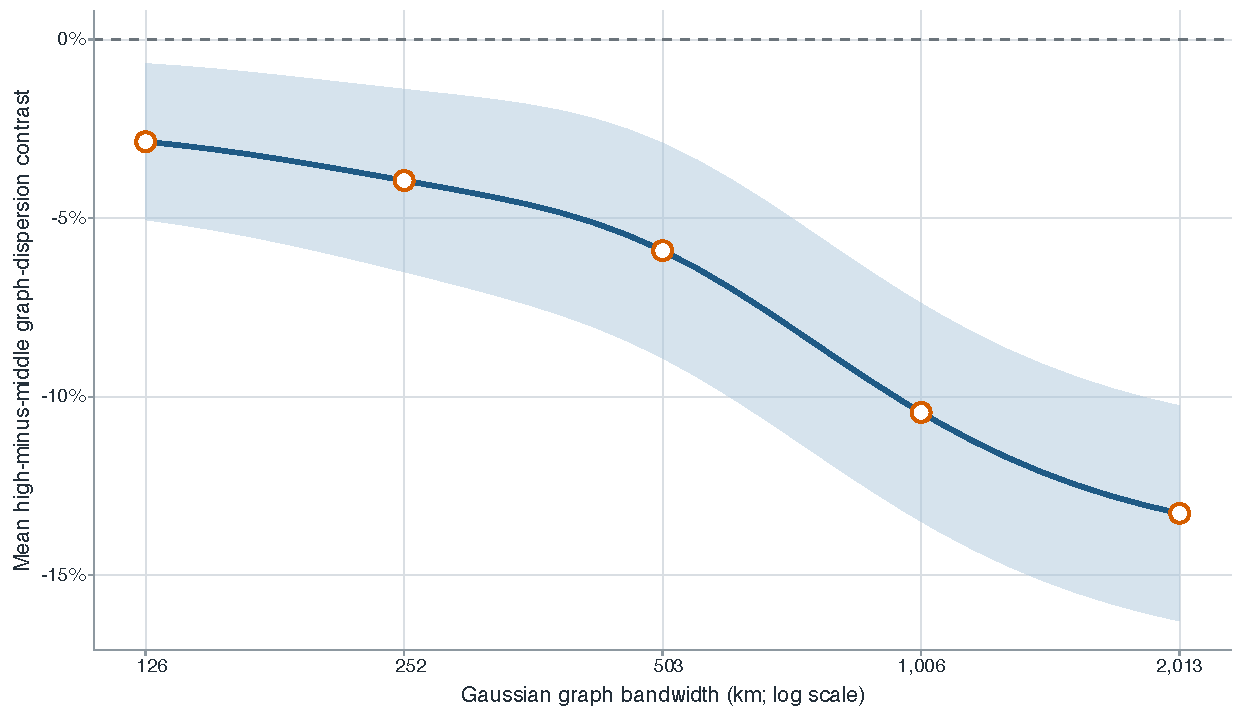
\includegraphics[width=0.92\textwidth]{supp_dense_bandwidth_profile.pdf}
\caption{Bandwidth-resolution profile on the 121-site support. The blue line
and shaded band show the 31-point profile and its pointwise 95\% intervals;
orange open circles mark the five prespecified bandwidths.}
\figalttext{A line descends smoothly as bandwidth increases
from 126 to 2,013 km. All 31 estimated effects are negative, and the five
prespecified bandwidths lie on the same monotone profile.}
\label{fig:dense-bandwidth}
\end{figure}

\subsection{Four spatial-support configurations}

The convergence comparison keeps the five physical bandwidths, primary peak times
and original 121-site labels fixed. The 239-site configuration refines
longitude while retaining the primary latitudes; the 236-site configuration
refines latitude while retaining the primary longitudes. Each contains every
primary site and is a subset of the 465-site grid, although the two
one-direction refinements are not nested within one another.

\begin{table}[htbp]
\centering
\caption{Four-configuration spatial-resolution comparison. Effects and the two
error summaries are in percentage points. Differences use the 465-site result
at the same fixed physical bandwidth as the reference.}
\label{tab:spatial-convergence}
\footnotesize
\setlength{\tabcolsep}{4pt}
\begin{tabular}{lrrrrrrrr}
\toprule
Configuration & Sites & 126 & 252 & 503 & 1,006 & 2,013 & Max.
$|\Delta|$ & RMSE \\
\midrule
Primary support & 121 & $-2.856$ & $-3.945$ & $-5.907$ & $-10.441$ & $-13.268$ & 0.991 & 0.764 \\
Longitude refined & 239 & $-2.839$ & $-3.846$ & $-5.968$ & $-10.552$ & $-13.351$ & 0.929 & 0.728 \\
Latitude refined & 236 & $-3.129$ & $-4.308$ & $-6.529$ & $-10.865$ & $-13.458$ & 0.500 & 0.384 \\
Dense support & 465 & $-3.395$ & $-4.543$ & $-6.898$ & $-11.340$ & $-13.959$ & 0.000 & 0.000 \\
\bottomrule
\end{tabular}
\end{table}

Every support retains the broad-to-local ordering and a negative effect at all
five bandwidths. Relative to 465 sites, the 121-site profile has a maximum
absolute discrepancy of 0.99 points and an across-scale RMSE of 0.76 points.
These finite-grid comparisons quantify sensitivity to the available spatial
support. Their scope is finite-support sensitivity, with continuous-domain
convergence left unassessed. Intersite spacing and the separate station
comparison provide the least support for the narrowest graph.

\begin{figure}[htbp]
\centering
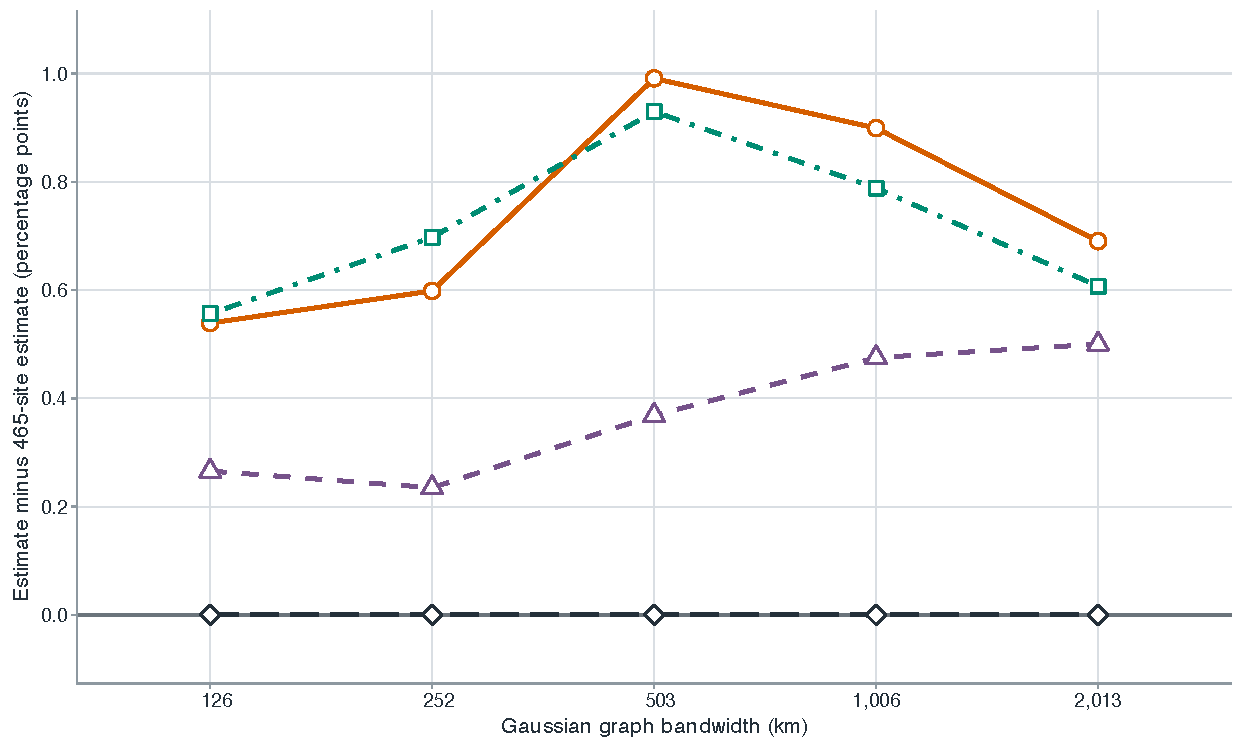
\includegraphics[width=0.92\textwidth]{supp_spatial_convergence.pdf}
\caption{Differences from the 465-site estimate at five fixed bandwidths.
Orange circles with a solid line denote the primary 121-site support; purple
triangles with a dashed line, the latitude-refined 236-site support; teal
squares with a dot-dash line, the longitude-refined 239-site support; and dark
diamonds with a long-dash line, the dense 465-site reference.}
\figalttext{Four lines compare each spatial support with the
465-site reference across five bandwidths. All differences are between zero
and one percentage point, and the broad-to-local ordering of the underlying
effects is unchanged.}
\label{fig:spatial-convergence}
\end{figure}

\section{Historical extension, 1950--1990}
\label{sec:historical-extension}

The ERA5-Land archive distributed through the Copernicus Climate Data Store
begins in January 1950.\footnote{Dataset overview:
\url{https://cds.climate.copernicus.eu/datasets/reanalysis-era5-land?tab=overview}.}
The historical-extension plan was finalised on 9 August 2026, after the
1991--2025 analysis and before retrieval of any 1950--1990 value. It specified
all 41 JJA summers, the same 121 sites, the five bandwidths and the original
quality control, Bolton wet-bulb calculation, UTC daily-peak rule and type-7
within-record quartiles. The analysis weights the three months, five scales
and summers equally. The extension is separated in calendar time from the
1991--2025 period, but both analyses share the ERA5-Land model and assimilation
system. The dated plan also specified one 99,999-draw joint product
cyclic-shift calculation with seed 20260810, with all five dispersion columns
rotated together within each historical month-year record.

The five-scale effect over 1950--1990 is $-11.04\%$ (95\% interval
$[-12.84,-9.24]\%$), with a negative estimate in 40 of 41
summers. Deleting one summer at a time gives estimates from $-11.33\%$ to
$-10.62\%$. Table~\ref{tab:historical-extension} gives the fixed period split
and the five-scale profile.

\begin{table}[htbp]
\centering
\caption{The 1950--1990 historical extension. Estimates and intervals
are percentages; the final column counts summers with a negative estimate.
Period rows average the five bandwidths. Scale rows use all 41 summers.}
\label{tab:historical-extension}
\small
\setlength{\tabcolsep}{7pt}
\begin{tabular}{lrrrr}
\toprule
Period or bandwidth & Summers & Estimate & 95\% interval & Negative summers \\
\midrule
1950--1990 overall & 41 & $-11.04$ & $[-12.84,-9.24]$ & 40 \\
1950--1978 & 29 & $-10.50$ & $[-12.50,-8.51]$ & 28 \\
1979--1990 & 12 & $-12.34$ & $[-16.65,-8.04]$ & 12 \\
\midrule
126 km   & 41 & $-5.96$  & $[-7.37,-4.54]$   & 38 \\
252 km   & 41 & $-7.51$  & $[-9.15,-5.87]$   & 39 \\
503 km   & 41 & $-10.08$ & $[-12.11,-8.04]$  & 40 \\
1,006 km & 41 & $-14.50$ & $[-16.72,-12.27]$ & 41 \\
2,013 km & 41 & $-17.17$ & $[-19.44,-14.91]$ & 41 \\
\bottomrule
\end{tabular}
\end{table}

Provider documentation identifies the forcing change used for the period
split: ERA5-Land for 1950--1978 used the preliminary ERA5 back extension,
whereas the later period used the consolidated ERA5 release.\footnote{ERA5-Land
production note:
\url{https://confluence.ecmwf.int/pages/viewpage.action?pageId=402639006}.}
Both period estimates are negative, and their intervals overlap. The
1950--1978 estimate inherits uncertainty from the preliminary forcing data.

As specified in the pre-access extension plan, we applied the product
cyclic-shift calculation to 123 month-year records, using $B=99{,}999$ joint
five-scale shifts and seed 20260810. None of the
sampled statistics was at or below the observed $-11.043\%$, so the plus-one
lower-tail value is 0.00001. The sampled null mean and standard deviation are
$0.853\%$ and $1.436$ percentage points. Every scale has an unadjusted value
of 0.00001; the complete-null single-step values range from 0.00001 to
0.00006.

For the exploratory historical climatology--anomaly decomposition, the monthly
reference field was estimated within 1950--1990:
\[
 \boldsymbol\mu_m^{H}=\frac{1}{41}\sum_{y=1950}^{1990}
 \left(\frac{1}{n_m}\sum_{t\in m}\mathbf y_{yt}\right),
 \qquad
 \mathbf a_{yt}^{H}=\mathbf y_{yt}-\boldsymbol\mu_m^{H}.
\]
Thus $\boldsymbol\mu_m^{H}$ is the site-specific mean field for month $m$
across the 41 historical summers. The anomaly and
alignment terms therefore describe departures from the historical period's
own persistent monthly spatial pattern.

Table~\ref{tab:historical-structure} reports the protocol-specified latitude
and planar accounting and the exploratory climatology--anomaly accounting for
the historical extension. The latitude and planar structured components are
negative in all 41 summers at every bandwidth. At 2,013 km, anomaly energy is
$-0.28$ points with interval $[-1.01,0.45]$, while the climatology--anomaly
alignment component is $-16.89$ points $[-19.31,-14.47]$ and is negative in
all 41 summers. Thus the broad-scale historical result has a low-dimensional
and alignment-dominated accounting pattern similar to that in the 1991--2025
period.

\begin{table}[htbp]
\centering
\caption{Structural accounting for the 1950--1990 extension. Entries are
percentage points. Within each geographic basis, the structured and residual
columns add to the total. The anomaly and alignment columns also add to the
total because the fixed climatology-energy difference is zero.}
\label{tab:historical-structure}
\scriptsize
\setlength{\tabcolsep}{4pt}
\begin{tabular}{rrrrrrrr}
\toprule
Bandwidth & Total & Latitude & Latitude & Planar & Planar & Anomaly & Climatology-- \\
(km) & effect & structured & residual & structured & residual & energy & anomaly alignment \\
\midrule
126   & $-5.96$  & $-2.83$  & $-3.13$ & $-3.15$  & $-2.81$ & $-3.22$ & $-2.74$ \\
252   & $-7.51$  & $-4.92$  & $-2.59$ & $-5.50$  & $-2.01$ & $-3.30$ & $-4.21$ \\
503   & $-10.08$ & $-8.86$  & $-1.21$ & $-9.92$  & $-0.15$ & $-2.41$ & $-7.67$ \\
1,006 & $-14.50$ & $-13.60$ & $-0.90$ & $-14.99$ & $+0.49$ & $-1.02$ & $-13.48$ \\
2,013 & $-17.17$ & $-16.13$ & $-1.05$ & $-17.62$ & $+0.44$ & $-0.28$ & $-16.89$ \\
\bottomrule
\end{tabular}
\end{table}

\section{NOAA station extension in ten evaluation years}
\label{sec:noaa-extension}

The station-extension plan was finalised on 9 August 2026 before retrieval of
the new station-year files or calculation of their high--middle effects. The
plan fixed the years by enumeration rather than by a rule applied to station
outcomes: 1992, 1996, 2000, 2004, 2008, 2012, 2016, 2020, 2023 and 2025. The
set can be written as $\{1992+4k:k=0,\ldots,7\}\cup\{2023,2025\}$. The protocol
defines the year set by this enumeration; station coverage and effect estimates
do not enter the choice. The 2015 and 2022 development years are excluded. We archived the
official Integrated Surface Database (ISD) station-history snapshot used for
selection.\footnote{NOAA Integrated Surface Database:
\url{https://www.ncei.noaa.gov/products/land-based-station/integrated-surface-database}.}
The planned eligibility rule required a station-history end date on or after
31 August 2025, but that snapshot contained no such candidate: its global
maximum end date was 28 August and its maximum inside the fixed study
rectangle was 24 August. The operational administrative cutoff was therefore
24 August. This outcome-blind metadata amendment was made before retrieval of
station WBT observations, matched ERA5-Land values or calculation of any graph
contrast. The year set, study rectangle, geographic proximity rule and target
sample size were unchanged.

For a candidate station $s$, the proximity criterion was
\[
 d(s,\mathcal S_{121})=\min_{i\in\mathcal S_{121}}d(s,i)\leq150\ \mathrm{km},
\]
where $\mathcal S_{121}$ is the fixed primary analysis support. For coordinate
differences in degrees, the pairwise distance was
\[
d(s,i)=\left[
 \{111.32\cos(\bar\phi_{si})(\lambda_s-\lambda_i)\}^{2}
 +\{110.57(\phi_s-\phi_i)\}^{2}
\right]^{1/2},
\]
with $\bar\phi_{si}$, the pair's mean latitude, converted to radians in the
cosine. This filter was
applied before maximin selection and kept station locations close to the
primary spatial support. Of the 228 stations satisfying the rectangle and date
conditions, 20 exceeded 150 km, leaving 208 candidates; the largest retained
nearest-site distance was 147.73 km and the smallest excluded distance was
155.72 km. A
deterministic maximin rule based on station coordinates selected 30 stations.
The study rectangle defined the candidate domain. A station-year qualified with at least 400 exact UTC
hours having temperature, dew point and usable station pressure; 26--30 of the
30 selected stations qualified in each year. We calculated station wet-bulb
temperature with the same Bolton implementation used for ERA5-Land.

The nearest ERA5-Land cells for the Shengsi and Taidong island stations had no
finite land values at any requested time. We recorded both point series as
unavailable. The other
28 station locations had finite ERA5-Land series. Combining this land-mask
restriction with the hourly qualification rule left 24--28 matched stations
per year and 175,172 paired hours. Table~\ref{tab:noaa-extension-measurement}
reports the measurement comparison. Bias is ERA5-Land minus station wet-bulb
temperature; the centred correlation subtracts each station mean before
pooling. The all-year row pools all matched hours across years.

\begin{table}[htbp]
\centering
\caption{ERA5-Land and NOAA station wet-bulb agreement in ten
evaluation years. Bias, MAE and RMSE are in $^\circ$C. Stations are the
qualified locations with a finite nearest-cell ERA5-Land series in that
year.}
\label{tab:noaa-extension-measurement}
\footnotesize
\setlength{\tabcolsep}{5pt}
\begin{tabular}{rrrrrrr}
\toprule
Year & Stations & Matched hours & Bias & MAE & RMSE & Centred correlation \\
\midrule
1992 & 25 & 17,887 & $-0.25$ & 0.88 & 1.16 & 0.919 \\
1996 & 25 & 19,147 & $-0.33$ & 0.88 & 1.16 & 0.908 \\
2000 & 25 & 16,765 & $-0.40$ & 0.94 & 1.21 & 0.908 \\
2004 & 25 & 16,829 & $-0.20$ & 0.91 & 1.18 & 0.923 \\
2008 & 25 & 17,310 & $-0.20$ & 0.88 & 1.14 & 0.909 \\
2012 & 25 & 17,349 & $-0.27$ & 0.93 & 1.22 & 0.918 \\
2016 & 24 & 16,589 & $-0.34$ & 0.88 & 1.13 & 0.937 \\
2020 & 28 & 19,323 & $-0.26$ & 1.04 & 1.48 & 0.897 \\
2023 & 27 & 16,554 & $-0.19$ & 1.02 & 1.49 & 0.925 \\
2025 & 28 & 17,419 & $-0.17$ & 1.01 & 1.45 & 0.933 \\
\midrule
All years & 28 & 175,172 & $-0.26$ & 0.94 & 1.27 & 0.916 \\
\bottomrule
\end{tabular}
\end{table}

For the effect comparison, ERA5-Land peak times and high/middle labels defined
the event days, and we aligned station observations to those events. Each
graph field used the same available station subset
for NOAA and ERA5-Land and required at least ten stations. All 30
month-year records retained at least one high and one middle field, giving
345 usable event fields. We formed a high-to-middle ratio within record,
averaged the three months equally within year and then averaged the ten years.
Table~\ref{tab:noaa-extension-effect} reports 95\% intervals. Inference focuses
on the 503-, 1,006- and 2,013-km graphs supported by the station spacing; the
two narrower graphs remain descriptive.

\begin{table}[H]
\centering
\caption{High--middle graph-dispersion effects at ERA5-Land-defined peak times
and labels in ten evaluation years. Effects and intervals are
percentages. ``Negative'' counts years with a negative scale-specific
estimate. Each scale contains all 30 month-year records and an average of
25.3 stations per event field.}
\label{tab:noaa-extension-effect}
\scriptsize
\setlength{\tabcolsep}{3pt}
\begin{tabularx}{\textwidth}{rYrYr}
\toprule
Bandwidth & NOAA effect [95\% interval] & NOAA negative & ERA5-Land effect [95\% interval] & ERA negative \\
(km) & & years & & years \\
\midrule
126   & $-6.23\ [-25.87,13.41]$ & 6/10 & $-11.60\ [-27.49,4.29]$    & 7/10 \\
252   & $-7.23\ [-21.01,6.55]$  & 7/10 & $-12.74\ [-22.68,-2.81]$  & 8/10 \\
503   & $-12.50\ [-24.05,-0.96]$ & 8/10 & $-17.13\ [-25.15,-9.11]$ & 10/10 \\
1,006 & $-18.03\ [-29.17,-6.90]$ & 9/10 & $-21.60\ [-29.07,-14.14]$ & 10/10 \\
2,013 & $-21.47\ [-32.51,-10.43]$ & 9/10 & $-24.23\ [-31.72,-16.74]$ & 10/10 \\
\bottomrule
\end{tabularx}
\end{table}

The station and paired ERA5-Land profiles are negative at all five scales and
become more negative with bandwidth. Averaging the three station-supported
scales within each year gives $-17.34\%$ (95\% interval
$[-28.49,-6.18]\%$), with a negative average in nine of ten years. The same
fixed broad-profile calculation for the matched ERA5-Land fields gives
$-20.99\%$ ($[-28.57,-13.40]\%$), negative in all ten years. These results
compare the two fields on identical, time-varying station supports. Because
ERA5-Land defines the event times and labels, this is an external measurement
and temporally separated effect comparison under a common event definition,
not an independent event replication. The irregularly sampled years, changing
qualified subsets and sparse support at 126 and 252 km limit the comparison.

\section{Continuous intensity and calendar matching}
\label{sec:intensity-calendar}

We evaluated two alternative event contrasts using the same sites, graphs and
aggregation hierarchy. For the continuous calculation, we
regressed $\log Q_h$ on centred regional wet-bulb temperature separately in
each month-year record. We then averaged slopes equally across months, scales
and the 33 evaluation summers. The five-scale mean slope is
$-0.0650\ {{}^\circ\mathrm C}^{-1}$, with a 95\% interval
of $[-0.0822,-0.0479]$ and negative summer slopes in 31 of 33 years.

The calendar-matched calculation compares each high day with the mean of
middle days no more than three or five calendar days away in the same
month-year record. We average eligible high-day contrasts within record
before applying the original equal-month, equal-scale and equal-summer
hierarchy. The $\pm3$-day window matches 670 of 792 high days (84.6\%); the
$\pm5$-day window matches 750 (94.7\%). Each of the 99 evaluation month-year
records contributes at least one match under both windows.

\begin{table}[htbp]
\centering
\caption{Continuous-intensity and calendar-matched results for the 33 evaluation
summers. Continuous entries are slopes of $\log Q_h$ per $^\circ$C. Matching
entries are percentage effects. Brackets give 95\% intervals.}
\label{tab:intensity-calendar}
\footnotesize
\setlength{\tabcolsep}{5pt}
\begin{tabularx}{\textwidth}{rYYY}
\toprule
Bandwidth & Continuous slope [interval] & $\pm3$-day match [interval] & $\pm5$-day match [interval] \\
\midrule
126   & $-0.0318\ [-0.0435,-0.0201]$ & $-2.32\ [-4.73,0.09]$   & $-2.54\ [-4.90,-0.18]$ \\
252   & $-0.0408\ [-0.0553,-0.0263]$ & $-3.29\ [-6.03,-0.56]$  & $-3.54\ [-6.18,-0.90]$ \\
503   & $-0.0546\ [-0.0735,-0.0356]$ & $-4.41\ [-7.44,-1.38]$  & $-4.74\ [-7.66,-1.83]$ \\
1,006 & $-0.0877\ [-0.1092,-0.0661]$ & $-7.17\ [-10.32,-4.02]$ & $-7.90\ [-10.94,-4.86]$ \\
2,013 & $-0.1104\ [-0.1325,-0.0882]$ & $-8.87\ [-12.06,-5.68]$ & $-9.89\ [-12.98,-6.80]$ \\
\midrule
Five-scale mean & $-0.0650\ [-0.0822,-0.0479]$ & $-5.21\ [-8.01,-2.41]$ & $-5.72\ [-8.43,-3.02]$ \\
\bottomrule
\end{tabularx}
\end{table}

The matched effects are weaker than the unrestricted high-to-middle contrast,
but their broad-to-local ordering remains. Calendar matching also changes the
target population of day pairs: only high days with eligible middle days enter
the high-day average.

\section{Heavy-tailed ratio stress test}
\label{sec:ratio-stress}

We compared the raw effect $r-1$, the log effect $\log r$ and the bounded
symmetric effect $2(r-1)/(r+1)$, where $r$ is the high-to-middle dispersion
ratio. The stress design uses the 121 observed site locations, exponential
spatial covariance with 450-km range and 5\% nugget, circular field
correlation 0.45 and regional-mean autoregression 0.65. A common daily scale
$\sqrt{3/\chi^2_3}$ produces heavy-tailed graph energy. Each scenario has
2,000 paired replications of six 30--31-day records. All three measures use
the same 999 product shifts within a replication; the seed is 20260811.

\begin{table}[htbp]
\centering
\caption{Raw, log and bounded effect measures under the heavy-tailed stress
design. Bias and RMSE are on each measure's scale. Size and power are
lower-tail rejection proportions at 0.05. Alternative targets correspond to
a high-day energy multiplier of 0.93.}
\label{tab:ratio-stress}
\scriptsize
\setlength{\tabcolsep}{3pt}
\begin{tabular}{lrrrrrrr}
\toprule
Measure & Null bias & Null RMSE & Size & Alternative target & Alt. bias & Alt. RMSE & Power \\
\midrule
Raw ratio         & $0.3716$  & $1.4725$ & $0.0470$ & $-0.0700$ & $0.3456$  & $1.3694$ & $0.0795$ \\
Log ratio         & $-0.0698$ & $0.3283$ & $0.0490$ & $-0.0726$ & $-0.0698$ & $0.3283$ & $0.0850$ \\
Bounded symmetric & $-0.0657$ & $0.2771$ & $0.0475$ & $-0.0725$ & $-0.0574$ & $0.2748$ & $0.0790$ \\
\bottomrule
\end{tabular}
\end{table}

The three product-shift tests retain near-nominal size in this design. The raw
ratio nevertheless has an RMSE more than five times that of the bounded
measure under the null. Randomisation validity governs label assignment for a
fixed statistic, whereas ratio-estimation stability also depends on the right
tail of daily energy. The log and bounded summaries reduce that instability,
with the bounded measure giving the smallest RMSE in these cells.

\section{Simulation specifications and results}
\label{sec:complete-simulations}

\subsection{Coupled label--field stress designs}

The coupled simulation uses the 121 observed site coordinates and six records
of lengths 30, 31, 30, 30, 31 and 30 days. Isotropic anomaly fields have
exponential covariance with 450-km range and 5\% nugget. The field state has
autoregressive coefficient 0.45, and the regional weather series has
coefficient 0.65. High and middle labels use type-7 quartiles within each
record. A standardised spatial gradient is proportional to $0.8x+y$, where
$x$ and $y$ are projected site coordinates. Its sign is driven by
$0.75\widetilde\mu_t+(1-0.75^2)^{1/2}Z_t$, so labels and spatial structure
share a latent weather component even under the null.

\begin{table}[htbp]
\centering
\caption{Exact changes defining the eight coupled label--field designs. Every
cell retains the common six-record construction and within-record labels.}
\label{tab:joint-dgp-specification}
\footnotesize
\setlength{\tabcolsep}{4pt}
\begin{tabularx}{\textwidth}{Z{0.22\textwidth}YY}
\toprule
Design & Null & Contraction alternative \\
\midrule
Shared latent gradient & Gradient amplitude is 1.8 on every day; its
sign shares the latent driver with regional weather. & Gradient amplitude on
high days is reduced from 1.8 to 1.2. \\

Within-month progression & Regional mean is a linear trend from $-1.4$ to
$1.4$ plus $0.60$ times the AR(1) weather series; gradient amplitude remains
1.8. & Gradient amplitude declines linearly from 1.95 to 1.30 across the
record. \\

Anisotropic covariance & Anomaly e-folding ranges are 800 km in projected
longitude and 300 km in projected latitude. & High-day anomaly amplitude is
multiplied by 0.94. \\

Peak-hour selection & Each daily regional mean is the maximum of 24 hourly
values with sinusoidal amplitude 1.8 and independent noise SD 0.35; anomaly
covariance is hour-invariant. & High-day anomaly amplitude is multiplied by
0.94. \\
\bottomrule
\end{tabularx}
\end{table}

Each field is evaluated with the five Gaussian graphs and a five-bin
variogram profile whose bins are the quintiles of the 7,260 observed pair
distances. For each replication, the target is the high-to-middle contrast in
the conditional expected quadratic forms. The graph and variogram statistics
use the same simulated fields, labels and product shifts. Each of the eight
cells contains 1,000 replications with 499 shifts per test.

\subsection{Repeated-summer experiment}

The annual experiment crosses
$R\in\{20,33,60,120\}$, $\rho\in\{0,0.3,0.6\}$, Gaussian, centred log-normal
and standardised $t_3$ innovations, and effects
$\delta\in\{0,-0.035,-0.07\}$. The resulting 108 cells each contain 10,000
replications after a 200-step burn-in. For retained summer $r$,
\[
 U_r=\rho U_{r-1}+(1-\rho^2)^{1/2}\varepsilon_r,
 \qquad Y_r=\delta+0.12U_r.
\]
The Gaussian innovation is standard normal. For $Z\sim N(0,1)$, the centred
unit-variance log-normal innovation is
\[
 \frac{\exp(0.65Z)-\exp(0.65^2/2)}
 {\{[\exp(0.65^2)-1]\exp(0.65^2)\}^{1/2}},
\]
and the heavy-tailed innovation is $T_3/\sqrt{3}$. The point estimate is
$\bar Y$. The ordinary interval uses the sample variance and a
$t_{R-1}$ critical value. The lag-2 calculation uses a Bartlett long-run
variance with the same critical value. The growing-lag interval uses
$L=\max\{1,\lfloor R^{1/3}\rfloor\}$ and a standard-normal critical value.
The sign test uses the exact binomial upper tail of the number of negative
summers. The three-test decision requires the Student, lag-2 and sign
$p$-values all to be at most 0.025. Standardised diagnostics use the known
long-run variance $0.12^2(1+\rho)/(1-\rho)$.

The following tables report all eight coupled cells and all 108 annual cells.

% Generated by code/46_prepare_supplement_simulation_tables.py
\begin{table}[H]
\centering
\caption{Complete results for the eight coupled label--field stress designs. Targets, bias and RMSE are percentage points; rejection is per cent over 1,000 replications. Graph and five-bin variogram profiles use identical fields, labels and product shifts.}
\label{tab:joint-dgp-complete}
\scriptsize
\setlength{\tabcolsep}{3.2pt}
\begin{tabular}{P{0.19\textwidth}P{0.13\textwidth}rrrrrrrr}
\toprule
Scenario & Family & \multicolumn{4}{c}{Graph profile} & \multicolumn{4}{c}{Five-bin variogram} \\
 & & Target & Bias & RMSE & Reject & Target & Bias & RMSE & Reject \\
\midrule
Shared-latent null & Null & 0.00 & 0.38 & 3.63 & 5.5 & -0.00 & 0.53 & 4.58 & 5.3 \\
Shared-latent contraction & Alternative & -27.37 & 0.19 & 2.70 & 100.0 & -36.66 & 0.25 & 3.26 & 100.0 \\
Seasonal-progression null & Null & 0.00 & 0.64 & 3.76 & 4.0 & -0.00 & 0.85 & 4.77 & 4.3 \\
Seasonal-gradient contraction & Alternative & -10.74 & 0.27 & 3.65 & 78.6 & -14.72 & 0.33 & 4.60 & 83.3 \\
Anisotropic null & Null & 0.00 & 0.31 & 3.86 & 7.0 & 0.00 & 0.42 & 4.81 & 7.3 \\
Anisotropic amplitude contraction & Alternative & -5.92 & 0.21 & 3.63 & 51.4 & -3.98 & 0.32 & 4.58 & 25.5 \\
Peak-selection null & Null & 0.00 & 0.21 & 3.69 & 6.6 & -0.00 & 0.34 & 4.63 & 6.6 \\
Peak-selection contraction & Alternative & -5.90 & 0.36 & 3.50 & 54.2 & -3.96 & 0.52 & 4.46 & 25.1 \\
\bottomrule
\end{tabular}
\end{table}

\scriptsize
\setlength{\tabcolsep}{3.5pt}
\begin{longtable}{rrllrrrrr}
\caption{Complete 108-cell repeated-summer results: estimation and coverage. Bias and RMSE are percentage points; coverage is per cent.}\label{tab:year-simulation-complete-a}\\
\toprule
$R$ & $\rho$ & Innovation & Effect & Bias & RMSE & Student & Lag 2 & Growing \\
 & & & & \multicolumn{2}{c}{percentage points} & \multicolumn{3}{c}{coverage (\%)} \\
\midrule
\endfirsthead
\multicolumn{9}{l}{\tablename\ \thetable\ continued}\\
\toprule
$R$ & $\rho$ & Innovation & Effect & Bias & RMSE & Student & Lag 2 & Growing \\
\midrule
\endhead
\midrule\multicolumn{9}{r}{Continued on next page}\\\endfoot
\bottomrule\endlastfoot
20 & 0.0 & Gaussian & Null & 0.015 & 2.655 & 95.4 & 91.7 & 89.9 \\
20 & 0.0 & Gaussian & $-3.5\%$ & -0.015 & 2.680 & 94.8 & 91.1 & 89.2 \\
20 & 0.0 & Gaussian & $-7\%$ & -0.015 & 2.665 & 95.1 & 91.3 & 89.4 \\
20 & 0.0 & Skewed & Null & -0.046 & 2.691 & 91.2 & 87.6 & 85.9 \\
20 & 0.0 & Skewed & $-3.5\%$ & 0.022 & 2.676 & 92.1 & 88.7 & 86.9 \\
20 & 0.0 & Skewed & $-7\%$ & -0.024 & 2.662 & 91.8 & 88.3 & 86.5 \\
20 & 0.0 & $t_3$ & Null & -0.028 & 2.672 & 95.3 & 91.7 & 89.7 \\
20 & 0.0 & $t_3$ & $-3.5\%$ & 0.028 & 2.599 & 95.9 & 92.0 & 90.4 \\
20 & 0.0 & $t_3$ & $-7\%$ & 0.028 & 2.696 & 95.9 & 92.0 & 90.1 \\
20 & 0.3 & Gaussian & Null & 0.081 & 3.584 & 85.5 & 86.8 & 84.8 \\
20 & 0.3 & Gaussian & $-3.5\%$ & -0.096 & 3.597 & 85.0 & 86.6 & 84.2 \\
20 & 0.3 & Gaussian & $-7\%$ & 0.036 & 3.620 & 85.0 & 86.5 & 84.0 \\
20 & 0.3 & Skewed & Null & 0.053 & 3.612 & 82.7 & 84.4 & 82.3 \\
20 & 0.3 & Skewed & $-3.5\%$ & 0.019 & 3.615 & 82.6 & 84.2 & 82.2 \\
20 & 0.3 & Skewed & $-7\%$ & -0.038 & 3.545 & 83.0 & 84.6 & 82.3 \\
20 & 0.3 & $t_3$ & Null & 0.056 & 3.486 & 85.9 & 87.5 & 85.1 \\
20 & 0.3 & $t_3$ & $-3.5\%$ & -0.126 & 3.533 & 85.7 & 87.3 & 84.8 \\
20 & 0.3 & $t_3$ & $-7\%$ & -0.002 & 3.620 & 85.8 & 87.8 & 85.3 \\
20 & 0.6 & Gaussian & Null & -0.042 & 5.096 & 66.5 & 76.2 & 73.4 \\
20 & 0.6 & Gaussian & $-3.5\%$ & 0.002 & 5.128 & 67.0 & 76.3 & 73.8 \\
20 & 0.6 & Gaussian & $-7\%$ & 0.000 & 5.175 & 66.6 & 75.9 & 73.2 \\
20 & 0.6 & Skewed & Null & 0.038 & 5.187 & 64.4 & 73.9 & 71.2 \\
20 & 0.6 & Skewed & $-3.5\%$ & -0.043 & 5.140 & 64.5 & 74.3 & 71.5 \\
20 & 0.6 & Skewed & $-7\%$ & -0.039 & 5.115 & 65.1 & 74.6 & 71.7 \\
20 & 0.6 & $t_3$ & Null & 0.047 & 4.987 & 65.9 & 76.3 & 73.5 \\
20 & 0.6 & $t_3$ & $-3.5\%$ & 0.075 & 5.101 & 65.1 & 75.8 & 72.7 \\
20 & 0.6 & $t_3$ & $-7\%$ & -0.026 & 5.254 & 65.5 & 76.7 & 73.7 \\
33 & 0.0 & Gaussian & Null & 0.057 & 2.065 & 95.2 & 93.3 & 91.2 \\
33 & 0.0 & Gaussian & $-3.5\%$ & -0.004 & 2.078 & 95.2 & 93.1 & 91.2 \\
33 & 0.0 & Gaussian & $-7\%$ & -0.021 & 2.062 & 95.2 & 93.5 & 91.4 \\
33 & 0.0 & Skewed & Null & -0.029 & 2.071 & 92.4 & 90.6 & 88.5 \\
33 & 0.0 & Skewed & $-3.5\%$ & -0.002 & 2.061 & 92.9 & 91.0 & 89.0 \\
33 & 0.0 & Skewed & $-7\%$ & 0.005 & 2.080 & 92.6 & 90.7 & 88.8 \\
33 & 0.0 & $t_3$ & Null & -0.019 & 2.089 & 95.8 & 93.7 & 91.5 \\
33 & 0.0 & $t_3$ & $-3.5\%$ & 0.007 & 2.062 & 95.6 & 93.2 & 91.0 \\
33 & 0.0 & $t_3$ & $-7\%$ & -0.004 & 2.127 & 95.7 & 93.6 & 91.5 \\
33 & 0.3 & Gaussian & Null & -0.046 & 2.837 & 85.4 & 89.0 & 87.3 \\
33 & 0.3 & Gaussian & $-3.5\%$ & -0.002 & 2.819 & 85.4 & 88.6 & 87.2 \\
33 & 0.3 & Gaussian & $-7\%$ & 0.018 & 2.808 & 85.7 & 88.8 & 87.3 \\
33 & 0.3 & Skewed & Null & 0.000 & 2.795 & 83.3 & 87.2 & 85.9 \\
33 & 0.3 & Skewed & $-3.5\%$ & -0.004 & 2.834 & 82.9 & 86.4 & 85.1 \\
33 & 0.3 & Skewed & $-7\%$ & -0.008 & 2.792 & 83.4 & 86.8 & 85.4 \\
33 & 0.3 & $t_3$ & Null & -0.011 & 2.773 & 85.0 & 89.2 & 87.5 \\
33 & 0.3 & $t_3$ & $-3.5\%$ & 0.012 & 2.804 & 85.5 & 89.4 & 88.2 \\
33 & 0.3 & $t_3$ & $-7\%$ & 0.033 & 2.760 & 85.4 & 89.1 & 87.8 \\
33 & 0.6 & Gaussian & Null & 0.004 & 4.112 & 66.1 & 78.7 & 79.0 \\
33 & 0.6 & Gaussian & $-3.5\%$ & 0.031 & 4.059 & 66.8 & 79.1 & 79.2 \\
33 & 0.6 & Gaussian & $-7\%$ & 0.027 & 4.049 & 67.3 & 79.5 & 79.6 \\
33 & 0.6 & Skewed & Null & 0.020 & 4.090 & 64.9 & 77.6 & 77.9 \\
33 & 0.6 & Skewed & $-3.5\%$ & 0.043 & 4.053 & 65.6 & 77.8 & 78.0 \\
33 & 0.6 & Skewed & $-7\%$ & 0.037 & 4.070 & 65.0 & 77.7 & 77.7 \\
33 & 0.6 & $t_3$ & Null & -0.014 & 3.994 & 66.5 & 79.8 & 80.1 \\
33 & 0.6 & $t_3$ & $-3.5\%$ & -0.054 & 4.004 & 66.0 & 79.9 & 80.3 \\
33 & 0.6 & $t_3$ & $-7\%$ & 0.006 & 4.158 & 65.4 & 79.6 & 79.8 \\
60 & 0.0 & Gaussian & Null & 0.002 & 1.554 & 95.1 & 94.0 & 92.9 \\
60 & 0.0 & Gaussian & $-3.5\%$ & -0.018 & 1.562 & 94.8 & 93.6 & 92.4 \\
60 & 0.0 & Gaussian & $-7\%$ & -0.003 & 1.551 & 95.0 & 93.8 & 92.8 \\
60 & 0.0 & Skewed & Null & -0.002 & 1.553 & 93.4 & 92.2 & 91.1 \\
60 & 0.0 & Skewed & $-3.5\%$ & 0.020 & 1.541 & 93.5 & 92.5 & 91.4 \\
60 & 0.0 & Skewed & $-7\%$ & 0.039 & 1.545 & 94.1 & 93.2 & 92.0 \\
60 & 0.0 & $t_3$ & Null & 0.019 & 1.583 & 95.4 & 94.3 & 93.2 \\
60 & 0.0 & $t_3$ & $-3.5\%$ & 0.008 & 1.523 & 95.5 & 94.3 & 93.3 \\
60 & 0.0 & $t_3$ & $-7\%$ & -0.008 & 1.536 & 95.7 & 94.8 & 93.6 \\
60 & 0.3 & Gaussian & Null & 0.016 & 2.097 & 85.0 & 90.0 & 89.7 \\
60 & 0.3 & Gaussian & $-3.5\%$ & -0.016 & 2.068 & 85.9 & 90.9 & 90.4 \\
60 & 0.3 & Gaussian & $-7\%$ & 0.033 & 2.083 & 85.6 & 90.6 & 90.3 \\
60 & 0.3 & Skewed & Null & -0.019 & 2.085 & 84.2 & 89.0 & 88.8 \\
60 & 0.3 & Skewed & $-3.5\%$ & 0.018 & 2.096 & 84.1 & 89.1 & 88.8 \\
60 & 0.3 & Skewed & $-7\%$ & -0.001 & 2.097 & 83.7 & 88.6 & 88.4 \\
60 & 0.3 & $t_3$ & Null & -0.014 & 2.082 & 85.2 & 90.5 & 90.0 \\
60 & 0.3 & $t_3$ & $-3.5\%$ & 0.035 & 2.088 & 84.7 & 90.7 & 90.3 \\
60 & 0.3 & $t_3$ & $-7\%$ & -0.010 & 2.087 & 85.1 & 90.5 & 90.1 \\
60 & 0.6 & Gaussian & Null & -0.011 & 3.056 & 67.0 & 81.0 & 82.5 \\
60 & 0.6 & Gaussian & $-3.5\%$ & -0.029 & 3.066 & 66.9 & 81.5 & 83.0 \\
60 & 0.6 & Gaussian & $-7\%$ & 0.030 & 3.036 & 67.3 & 81.3 & 82.8 \\
60 & 0.6 & Skewed & Null & 0.009 & 3.026 & 65.9 & 80.1 & 81.5 \\
60 & 0.6 & Skewed & $-3.5\%$ & -0.016 & 3.062 & 65.4 & 79.9 & 81.5 \\
60 & 0.6 & Skewed & $-7\%$ & -0.018 & 3.038 & 66.5 & 80.2 & 81.6 \\
60 & 0.6 & $t_3$ & Null & -0.003 & 2.988 & 66.1 & 81.0 & 82.6 \\
60 & 0.6 & $t_3$ & $-3.5\%$ & 0.005 & 3.063 & 66.6 & 81.3 & 82.9 \\
60 & 0.6 & $t_3$ & $-7\%$ & 0.026 & 3.046 & 66.0 & 81.5 & 83.0 \\
120 & 0.0 & Gaussian & Null & 0.013 & 1.098 & 94.8 & 94.3 & 93.7 \\
120 & 0.0 & Gaussian & $-3.5\%$ & 0.003 & 1.100 & 94.9 & 94.4 & 93.7 \\
120 & 0.0 & Gaussian & $-7\%$ & 0.023 & 1.101 & 94.7 & 94.2 & 93.2 \\
120 & 0.0 & Skewed & Null & 0.011 & 1.091 & 94.4 & 93.7 & 93.0 \\
120 & 0.0 & Skewed & $-3.5\%$ & 0.003 & 1.084 & 94.2 & 93.5 & 93.1 \\
120 & 0.0 & Skewed & $-7\%$ & -0.004 & 1.101 & 93.7 & 93.3 & 92.5 \\
120 & 0.0 & $t_3$ & Null & 0.008 & 1.115 & 95.2 & 94.5 & 93.9 \\
120 & 0.0 & $t_3$ & $-3.5\%$ & -0.007 & 1.099 & 95.2 & 94.4 & 93.8 \\
120 & 0.0 & $t_3$ & $-7\%$ & 0.004 & 1.100 & 95.5 & 94.8 & 94.0 \\
120 & 0.3 & Gaussian & Null & 0.013 & 1.493 & 84.8 & 90.8 & 91.5 \\
120 & 0.3 & Gaussian & $-3.5\%$ & 0.001 & 1.471 & 85.6 & 91.2 & 91.8 \\
120 & 0.3 & Gaussian & $-7\%$ & 0.002 & 1.489 & 84.8 & 90.9 & 91.5 \\
120 & 0.3 & Skewed & Null & -0.004 & 1.502 & 83.6 & 89.6 & 90.2 \\
120 & 0.3 & Skewed & $-3.5\%$ & -0.014 & 1.485 & 84.7 & 90.2 & 90.7 \\
120 & 0.3 & Skewed & $-7\%$ & 0.025 & 1.491 & 84.2 & 90.0 & 90.4 \\
120 & 0.3 & $t_3$ & Null & -0.009 & 1.495 & 84.7 & 91.1 & 91.7 \\
120 & 0.3 & $t_3$ & $-3.5\%$ & -0.028 & 1.475 & 84.6 & 91.2 & 91.7 \\
120 & 0.3 & $t_3$ & $-7\%$ & -0.002 & 1.488 & 84.5 & 90.7 & 91.4 \\
120 & 0.6 & Gaussian & Null & -0.018 & 2.164 & 67.9 & 82.8 & 86.5 \\
120 & 0.6 & Gaussian & $-3.5\%$ & -0.010 & 2.171 & 67.8 & 82.7 & 86.6 \\
120 & 0.6 & Gaussian & $-7\%$ & 0.023 & 2.169 & 66.9 & 82.3 & 86.5 \\
120 & 0.6 & Skewed & Null & -0.012 & 2.162 & 67.2 & 81.8 & 85.6 \\
120 & 0.6 & Skewed & $-3.5\%$ & -0.020 & 2.181 & 65.7 & 81.3 & 85.6 \\
120 & 0.6 & Skewed & $-7\%$ & 0.014 & 2.180 & 66.5 & 81.6 & 85.5 \\
120 & 0.6 & $t_3$ & Null & -0.013 & 2.184 & 66.6 & 82.5 & 86.4 \\
120 & 0.6 & $t_3$ & $-3.5\%$ & -0.053 & 2.146 & 66.5 & 82.5 & 86.6 \\
120 & 0.6 & $t_3$ & $-7\%$ & 0.015 & 2.180 & 65.7 & 82.2 & 86.3 \\
\end{longtable}

\scriptsize
\setlength{\tabcolsep}{4.5pt}
\begin{longtable}{rrllrrrr}
\caption{Complete 108-cell repeated-summer results: standardised-mean diagnostics. $L$ is the growing Bartlett lag; the standardised columns use the known long-run variance.}\label{tab:year-simulation-complete-b}\\
\toprule
$R$ & $\rho$ & Innovation & Effect & $L$ & $z$ mean & $z$ SD & $z_{.025},z_{.975}$ \\
\midrule
\endfirsthead
\multicolumn{8}{l}{\tablename\ \thetable\ continued}\\
\toprule
$R$ & $\rho$ & Innovation & Effect & $L$ & $z$ mean & $z$ SD & $z_{.025},z_{.975}$ \\
\midrule
\endhead
\midrule\multicolumn{8}{r}{Continued on next page}\\\endfoot
\bottomrule\endlastfoot
20 & 0.0 & Gaussian & Null & 2 & 0.006 & 0.990 & -1.94, 1.98 \\
20 & 0.0 & Gaussian & $-3.5\%$ & 2 & -0.006 & 0.999 & -1.98, 1.98 \\
20 & 0.0 & Gaussian & $-7\%$ & 2 & -0.006 & 0.993 & -1.92, 1.99 \\
20 & 0.0 & Skewed & Null & 2 & -0.017 & 1.003 & -1.71, 2.21 \\
20 & 0.0 & Skewed & $-3.5\%$ & 2 & 0.008 & 0.997 & -1.71, 2.18 \\
20 & 0.0 & Skewed & $-7\%$ & 2 & -0.009 & 0.992 & -1.68, 2.14 \\
20 & 0.0 & $t_3$ & Null & 2 & -0.010 & 0.996 & -1.92, 1.95 \\
20 & 0.0 & $t_3$ & $-3.5\%$ & 2 & 0.011 & 0.968 & -1.90, 1.90 \\
20 & 0.0 & $t_3$ & $-7\%$ & 2 & 0.010 & 1.005 & -1.88, 1.91 \\
20 & 0.3 & Gaussian & Null & 2 & 0.022 & 0.980 & -1.91, 1.94 \\
20 & 0.3 & Gaussian & $-3.5\%$ & 2 & -0.026 & 0.983 & -1.96, 1.93 \\
20 & 0.3 & Gaussian & $-7\%$ & 2 & 0.010 & 0.990 & -1.93, 1.92 \\
20 & 0.3 & Skewed & Null & 2 & 0.014 & 0.988 & -1.66, 2.18 \\
20 & 0.3 & Skewed & $-3.5\%$ & 2 & 0.005 & 0.989 & -1.68, 2.17 \\
20 & 0.3 & Skewed & $-7\%$ & 2 & -0.010 & 0.969 & -1.68, 2.12 \\
20 & 0.3 & $t_3$ & Null & 2 & 0.015 & 0.953 & -1.85, 1.91 \\
20 & 0.3 & $t_3$ & $-3.5\%$ & 2 & -0.035 & 0.966 & -1.94, 1.85 \\
20 & 0.3 & $t_3$ & $-7\%$ & 2 & -0.001 & 0.990 & -1.92, 1.91 \\
20 & 0.6 & Gaussian & Null & 2 & -0.008 & 0.950 & -1.89, 1.83 \\
20 & 0.6 & Gaussian & $-3.5\%$ & 2 & 0.000 & 0.956 & -1.89, 1.85 \\
20 & 0.6 & Gaussian & $-7\%$ & 2 & 0.000 & 0.964 & -1.91, 1.88 \\
20 & 0.6 & Skewed & Null & 2 & 0.007 & 0.967 & -1.64, 2.10 \\
20 & 0.6 & Skewed & $-3.5\%$ & 2 & -0.008 & 0.958 & -1.62, 2.11 \\
20 & 0.6 & Skewed & $-7\%$ & 2 & -0.007 & 0.953 & -1.60, 2.11 \\
20 & 0.6 & $t_3$ & Null & 2 & 0.009 & 0.929 & -1.77, 1.81 \\
20 & 0.6 & $t_3$ & $-3.5\%$ & 2 & 0.014 & 0.950 & -1.81, 1.87 \\
20 & 0.6 & $t_3$ & $-7\%$ & 2 & -0.005 & 0.979 & -1.84, 1.79 \\
33 & 0.0 & Gaussian & Null & 3 & 0.027 & 0.988 & -1.92, 1.97 \\
33 & 0.0 & Gaussian & $-3.5\%$ & 3 & -0.002 & 0.995 & -1.95, 1.92 \\
33 & 0.0 & Gaussian & $-7\%$ & 3 & -0.010 & 0.987 & -1.93, 1.93 \\
33 & 0.0 & Skewed & Null & 3 & -0.014 & 0.991 & -1.75, 2.12 \\
33 & 0.0 & Skewed & $-3.5\%$ & 3 & -0.001 & 0.987 & -1.72, 2.11 \\
33 & 0.0 & Skewed & $-7\%$ & 3 & 0.002 & 0.996 & -1.73, 2.13 \\
33 & 0.0 & $t_3$ & Null & 3 & -0.009 & 1.000 & -1.93, 1.92 \\
33 & 0.0 & $t_3$ & $-3.5\%$ & 3 & 0.003 & 0.987 & -1.93, 1.93 \\
33 & 0.0 & $t_3$ & $-7\%$ & 3 & -0.002 & 1.018 & -1.94, 1.91 \\
33 & 0.3 & Gaussian & Null & 3 & -0.016 & 0.996 & -1.99, 1.95 \\
33 & 0.3 & Gaussian & $-3.5\%$ & 3 & -0.001 & 0.990 & -1.93, 1.94 \\
33 & 0.3 & Gaussian & $-7\%$ & 3 & 0.006 & 0.987 & -1.92, 1.92 \\
33 & 0.3 & Skewed & Null & 3 & 0.000 & 0.982 & -1.72, 2.11 \\
33 & 0.3 & Skewed & $-3.5\%$ & 3 & -0.001 & 0.995 & -1.71, 2.13 \\
33 & 0.3 & Skewed & $-7\%$ & 3 & -0.003 & 0.981 & -1.73, 2.09 \\
33 & 0.3 & $t_3$ & Null & 3 & -0.004 & 0.974 & -1.93, 1.89 \\
33 & 0.3 & $t_3$ & $-3.5\%$ & 3 & 0.004 & 0.985 & -1.92, 1.94 \\
33 & 0.3 & $t_3$ & $-7\%$ & 3 & 0.012 & 0.970 & -1.94, 1.91 \\
33 & 0.6 & Gaussian & Null & 3 & 0.001 & 0.984 & -1.92, 1.92 \\
33 & 0.6 & Gaussian & $-3.5\%$ & 3 & 0.008 & 0.972 & -1.89, 1.87 \\
33 & 0.6 & Gaussian & $-7\%$ & 3 & 0.006 & 0.969 & -1.90, 1.88 \\
33 & 0.6 & Skewed & Null & 3 & 0.005 & 0.979 & -1.70, 2.12 \\
33 & 0.6 & Skewed & $-3.5\%$ & 3 & 0.010 & 0.970 & -1.68, 2.10 \\
33 & 0.6 & Skewed & $-7\%$ & 3 & 0.009 & 0.974 & -1.68, 2.09 \\
33 & 0.6 & $t_3$ & Null & 3 & -0.003 & 0.956 & -1.87, 1.83 \\
33 & 0.6 & $t_3$ & $-3.5\%$ & 3 & -0.013 & 0.958 & -1.89, 1.82 \\
33 & 0.6 & $t_3$ & $-7\%$ & 3 & 0.001 & 0.995 & -1.96, 1.88 \\
60 & 0.0 & Gaussian & Null & 3 & 0.001 & 1.003 & -1.93, 1.95 \\
60 & 0.0 & Gaussian & $-3.5\%$ & 3 & -0.012 & 1.008 & -2.01, 1.94 \\
60 & 0.0 & Gaussian & $-7\%$ & 3 & -0.002 & 1.001 & -1.94, 1.98 \\
60 & 0.0 & Skewed & Null & 3 & -0.001 & 1.003 & -1.79, 2.10 \\
60 & 0.0 & Skewed & $-3.5\%$ & 3 & 0.013 & 0.995 & -1.79, 2.09 \\
60 & 0.0 & Skewed & $-7\%$ & 3 & 0.025 & 0.997 & -1.78, 2.15 \\
60 & 0.0 & $t_3$ & Null & 3 & 0.013 & 1.022 & -1.96, 2.01 \\
60 & 0.0 & $t_3$ & $-3.5\%$ & 3 & 0.005 & 0.983 & -1.92, 1.96 \\
60 & 0.0 & $t_3$ & $-7\%$ & 3 & -0.005 & 0.991 & -1.89, 1.92 \\
60 & 0.3 & Gaussian & Null & 3 & 0.008 & 0.993 & -1.99, 1.92 \\
60 & 0.3 & Gaussian & $-3.5\%$ & 3 & -0.007 & 0.979 & -1.92, 1.90 \\
60 & 0.3 & Gaussian & $-7\%$ & 3 & 0.015 & 0.986 & -1.91, 1.91 \\
60 & 0.3 & Skewed & Null & 3 & -0.009 & 0.988 & -1.81, 2.07 \\
60 & 0.3 & Skewed & $-3.5\%$ & 3 & 0.008 & 0.993 & -1.78, 2.13 \\
60 & 0.3 & Skewed & $-7\%$ & 3 & -0.001 & 0.993 & -1.83, 2.08 \\
60 & 0.3 & $t_3$ & Null & 3 & -0.007 & 0.986 & -1.92, 1.98 \\
60 & 0.3 & $t_3$ & $-3.5\%$ & 3 & 0.017 & 0.989 & -1.91, 1.96 \\
60 & 0.3 & $t_3$ & $-7\%$ & 3 & -0.005 & 0.988 & -1.96, 1.95 \\
60 & 0.6 & Gaussian & Null & 3 & -0.003 & 0.986 & -1.92, 1.94 \\
60 & 0.6 & Gaussian & $-3.5\%$ & 3 & -0.009 & 0.989 & -1.96, 1.90 \\
60 & 0.6 & Gaussian & $-7\%$ & 3 & 0.010 & 0.980 & -1.89, 1.92 \\
60 & 0.6 & Skewed & Null & 3 & 0.003 & 0.977 & -1.78, 2.06 \\
60 & 0.6 & Skewed & $-3.5\%$ & 3 & -0.005 & 0.988 & -1.77, 2.10 \\
60 & 0.6 & Skewed & $-7\%$ & 3 & -0.006 & 0.980 & -1.76, 2.05 \\
60 & 0.6 & $t_3$ & Null & 3 & -0.001 & 0.964 & -1.90, 1.87 \\
60 & 0.6 & $t_3$ & $-3.5\%$ & 3 & 0.002 & 0.989 & -1.89, 1.92 \\
60 & 0.6 & $t_3$ & $-7\%$ & 3 & 0.008 & 0.983 & -1.94, 1.92 \\
120 & 0.0 & Gaussian & Null & 4 & 0.012 & 1.003 & -1.98, 1.97 \\
120 & 0.0 & Gaussian & $-3.5\%$ & 4 & 0.002 & 1.004 & -1.93, 1.99 \\
120 & 0.0 & Gaussian & $-7\%$ & 4 & 0.021 & 1.005 & -1.94, 2.02 \\
120 & 0.0 & Skewed & Null & 4 & 0.010 & 0.996 & -1.82, 2.07 \\
120 & 0.0 & Skewed & $-3.5\%$ & 4 & 0.003 & 0.989 & -1.86, 2.05 \\
120 & 0.0 & Skewed & $-7\%$ & 4 & -0.003 & 1.005 & -1.88, 2.07 \\
120 & 0.0 & $t_3$ & Null & 4 & 0.007 & 1.018 & -1.95, 2.01 \\
120 & 0.0 & $t_3$ & $-3.5\%$ & 4 & -0.006 & 1.003 & -1.96, 1.96 \\
120 & 0.0 & $t_3$ & $-7\%$ & 4 & 0.004 & 1.004 & -1.92, 2.02 \\
120 & 0.3 & Gaussian & Null & 4 & 0.008 & 1.000 & -1.98, 1.95 \\
120 & 0.3 & Gaussian & $-3.5\%$ & 4 & 0.001 & 0.986 & -1.92, 1.94 \\
120 & 0.3 & Gaussian & $-7\%$ & 4 & 0.001 & 0.997 & -1.94, 1.95 \\
120 & 0.3 & Skewed & Null & 4 & -0.003 & 1.006 & -1.86, 2.10 \\
120 & 0.3 & Skewed & $-3.5\%$ & 4 & -0.009 & 0.995 & -1.87, 2.06 \\
120 & 0.3 & Skewed & $-7\%$ & 4 & 0.017 & 0.999 & -1.82, 2.06 \\
120 & 0.3 & $t_3$ & Null & 4 & -0.006 & 1.001 & -1.94, 1.93 \\
120 & 0.3 & $t_3$ & $-3.5\%$ & 4 & -0.018 & 0.988 & -1.95, 1.94 \\
120 & 0.3 & $t_3$ & $-7\%$ & 4 & -0.001 & 0.997 & -1.98, 1.94 \\
120 & 0.6 & Gaussian & Null & 4 & -0.008 & 0.988 & -1.97, 1.95 \\
120 & 0.6 & Gaussian & $-3.5\%$ & 4 & -0.005 & 0.991 & -1.97, 1.94 \\
120 & 0.6 & Gaussian & $-7\%$ & 4 & 0.010 & 0.990 & -1.92, 1.93 \\
120 & 0.6 & Skewed & Null & 4 & -0.005 & 0.987 & -1.83, 2.09 \\
120 & 0.6 & Skewed & $-3.5\%$ & 4 & -0.009 & 0.996 & -1.85, 2.06 \\
120 & 0.6 & Skewed & $-7\%$ & 4 & 0.006 & 0.995 & -1.82, 2.08 \\
120 & 0.6 & $t_3$ & Null & 4 & -0.006 & 0.997 & -1.87, 1.91 \\
120 & 0.6 & $t_3$ & $-3.5\%$ & 4 & -0.024 & 0.979 & -1.97, 1.90 \\
120 & 0.6 & $t_3$ & $-7\%$ & 4 & 0.007 & 0.995 & -1.95, 1.93 \\
\end{longtable}

\scriptsize
\setlength{\tabcolsep}{4.5pt}
\begin{longtable}{rrllrrrrr}
\caption{Complete 108-cell repeated-summer results: one-sided rejection percentages. For Student, lag-2 and growing-lag tests, null rows estimate mean-null size and non-null rows estimate power. The sign calculation targets $\Pr(Y_r<0)=1/2$; under centred skewed mean-null innovations, its rejection rate quantifies departure from the sign null. The three-test column requires Student, lag-2 and sign values all to be at most 0.025.}\label{tab:year-simulation-complete-c}\\
\toprule
$R$ & $\rho$ & Innovation & Effect & Student & Lag 2 & Growing & Sign & Three-test \\
\midrule
\endfirsthead
\multicolumn{9}{l}{\tablename\ \thetable\ continued}\\
\toprule
$R$ & $\rho$ & Innovation & Effect & Student & Lag 2 & Growing & Sign & Three-test \\
\midrule
\endhead
\midrule\multicolumn{9}{r}{Continued on next page}\\\endfoot
\bottomrule\endlastfoot
20 & 0.0 & Gaussian & Null & 4.6 & 7.1 & 8.0 & 2.1 & 1.0 \\
20 & 0.0 & Gaussian & $-3.5\%$ & 34.8 & 40.7 & 43.6 & 15.8 & 12.1 \\
20 & 0.0 & Gaussian & $-7\%$ & 81.0 & 84.3 & 86.2 & 49.5 & 46.4 \\
20 & 0.0 & Skewed & Null & 11.8 & 14.6 & 15.6 & 19.0 & 6.3 \\
20 & 0.0 & Skewed & $-3.5\%$ & 45.4 & 49.5 & 51.6 & 53.8 & 31.2 \\
20 & 0.0 & Skewed & $-7\%$ & 77.3 & 80.3 & 81.5 & 82.9 & 64.7 \\
20 & 0.0 & $t_3$ & Null & 5.2 & 7.5 & 8.4 & 2.2 & 0.9 \\
20 & 0.0 & $t_3$ & $-3.5\%$ & 43.9 & 49.8 & 52.3 & 32.7 & 21.2 \\
20 & 0.0 & $t_3$ & $-7\%$ & 85.7 & 87.7 & 88.8 & 82.8 & 71.0 \\
20 & 0.3 & Gaussian & Null & 10.5 & 9.3 & 10.4 & 4.8 & 3.1 \\
20 & 0.3 & Gaussian & $-3.5\%$ & 41.0 & 37.6 & 39.9 & 21.9 & 17.9 \\
20 & 0.3 & Gaussian & $-7\%$ & 74.5 & 70.5 & 72.6 & 51.0 & 46.9 \\
20 & 0.3 & Skewed & Null & 17.4 & 16.5 & 17.6 & 20.3 & 10.3 \\
20 & 0.3 & Skewed & $-3.5\%$ & 47.8 & 44.6 & 46.3 & 50.9 & 33.3 \\
20 & 0.3 & Skewed & $-7\%$ & 75.2 & 72.7 & 74.1 & 77.2 & 62.1 \\
20 & 0.3 & $t_3$ & Null & 11.3 & 10.0 & 11.0 & 5.5 & 3.1 \\
20 & 0.3 & $t_3$ & $-3.5\%$ & 48.8 & 44.7 & 46.9 & 35.2 & 25.9 \\
20 & 0.3 & $t_3$ & $-7\%$ & 81.3 & 78.0 & 79.7 & 75.4 & 64.6 \\
20 & 0.6 & Gaussian & Null & 20.8 & 15.9 & 17.1 & 11.8 & 9.3 \\
20 & 0.6 & Gaussian & $-3.5\%$ & 44.4 & 36.0 & 37.7 & 28.7 & 24.2 \\
20 & 0.6 & Gaussian & $-7\%$ & 70.2 & 62.0 & 63.8 & 52.5 & 47.9 \\
20 & 0.6 & Skewed & Null & 27.0 & 22.1 & 23.0 & 24.1 & 16.9 \\
20 & 0.6 & Skewed & $-3.5\%$ & 51.7 & 44.9 & 46.5 & 47.2 & 36.5 \\
20 & 0.6 & Skewed & $-7\%$ & 71.8 & 65.3 & 66.7 & 68.5 & 57.1 \\
20 & 0.6 & $t_3$ & Null & 21.5 & 16.0 & 17.2 & 12.6 & 9.4 \\
20 & 0.6 & $t_3$ & $-3.5\%$ & 49.2 & 40.8 & 42.4 & 36.9 & 29.6 \\
20 & 0.6 & $t_3$ & $-7\%$ & 76.2 & 68.8 & 70.4 & 66.9 & 58.6 \\
33 & 0.0 & Gaussian & Null & 4.8 & 6.0 & 7.1 & 3.6 & 0.8 \\
33 & 0.0 & Gaussian & $-3.5\%$ & 49.6 & 53.2 & 56.3 & 33.8 & 18.1 \\
33 & 0.0 & Gaussian & $-7\%$ & 95.0 & 95.6 & 96.1 & 81.4 & 68.5 \\
33 & 0.0 & Skewed & Null & 10.3 & 12.0 & 13.3 & 39.3 & 5.9 \\
33 & 0.0 & Skewed & $-3.5\%$ & 55.5 & 58.1 & 60.6 & 84.7 & 42.7 \\
33 & 0.0 & Skewed & $-7\%$ & 89.0 & 89.8 & 90.8 & 98.4 & 81.8 \\
33 & 0.0 & $t_3$ & Null & 5.0 & 6.5 & 7.8 & 4.0 & 0.7 \\
33 & 0.0 & $t_3$ & $-3.5\%$ & 58.2 & 61.0 & 63.6 & 62.0 & 33.2 \\
33 & 0.0 & $t_3$ & $-7\%$ & 94.4 & 94.9 & 95.6 & 98.3 & 87.9 \\
33 & 0.3 & Gaussian & Null & 11.8 & 9.1 & 9.9 & 8.2 & 3.0 \\
33 & 0.3 & Gaussian & $-3.5\%$ & 50.5 & 44.1 & 45.3 & 37.0 & 23.0 \\
33 & 0.3 & Gaussian & $-7\%$ & 89.2 & 85.1 & 85.5 & 77.5 & 63.8 \\
33 & 0.3 & Skewed & Null & 17.1 & 14.4 & 14.9 & 36.5 & 9.4 \\
33 & 0.3 & Skewed & $-3.5\%$ & 55.7 & 50.7 & 51.6 & 76.8 & 40.7 \\
33 & 0.3 & Skewed & $-7\%$ & 85.2 & 81.8 & 82.3 & 95.2 & 74.7 \\
33 & 0.3 & $t_3$ & Null & 11.7 & 9.3 & 10.0 & 9.1 & 3.3 \\
33 & 0.3 & $t_3$ & $-3.5\%$ & 57.8 & 51.2 & 52.2 & 57.5 & 33.7 \\
33 & 0.3 & $t_3$ & $-7\%$ & 90.7 & 87.9 & 88.2 & 94.3 & 79.5 \\
33 & 0.6 & Gaussian & Null & 21.2 & 14.4 & 14.1 & 15.9 & 8.5 \\
33 & 0.6 & Gaussian & $-3.5\%$ & 50.8 & 40.2 & 39.4 & 41.1 & 27.8 \\
33 & 0.6 & Gaussian & $-7\%$ & 80.7 & 72.4 & 71.4 & 71.5 & 59.2 \\
33 & 0.6 & Skewed & Null & 26.1 & 20.0 & 19.5 & 34.3 & 14.9 \\
33 & 0.6 & Skewed & $-3.5\%$ & 55.5 & 46.7 & 45.9 & 65.2 & 39.0 \\
33 & 0.6 & Skewed & $-7\%$ & 79.5 & 72.0 & 71.2 & 85.6 & 65.1 \\
33 & 0.6 & $t_3$ & Null & 21.6 & 14.4 & 14.1 & 16.5 & 8.1 \\
33 & 0.6 & $t_3$ & $-3.5\%$ & 56.9 & 46.7 & 45.8 & 52.6 & 34.8 \\
33 & 0.6 & $t_3$ & $-7\%$ & 84.8 & 77.6 & 76.8 & 84.6 & 68.4 \\
60 & 0.0 & Gaussian & Null & 5.0 & 5.8 & 6.5 & 4.9 & 0.8 \\
60 & 0.0 & Gaussian & $-3.5\%$ & 71.8 & 73.6 & 74.7 & 54.4 & 31.7 \\
60 & 0.0 & Gaussian & $-7\%$ & 99.7 & 99.7 & 99.7 & 96.8 & 90.7 \\
60 & 0.0 & Skewed & Null & 9.2 & 10.0 & 10.6 & 62.6 & 5.2 \\
60 & 0.0 & Skewed & $-3.5\%$ & 70.6 & 71.7 & 72.7 & 98.3 & 59.5 \\
60 & 0.0 & Skewed & $-7\%$ & 97.6 & 97.7 & 97.9 & 100.0 & 95.5 \\
60 & 0.0 & $t_3$ & Null & 4.7 & 5.5 & 6.2 & 4.7 & 0.5 \\
60 & 0.0 & $t_3$ & $-3.5\%$ & 77.5 & 78.2 & 79.1 & 87.0 & 57.0 \\
60 & 0.0 & $t_3$ & $-7\%$ & 98.8 & 98.7 & 98.8 & 100.0 & 97.6 \\
60 & 0.3 & Gaussian & Null & 11.2 & 8.2 & 8.3 & 8.9 & 2.8 \\
60 & 0.3 & Gaussian & $-3.5\%$ & 67.5 & 59.5 & 59.4 & 54.2 & 33.7 \\
60 & 0.3 & Gaussian & $-7\%$ & 98.4 & 97.0 & 96.9 & 93.9 & 86.0 \\
60 & 0.3 & Skewed & Null & 15.2 & 11.9 & 12.1 & 52.5 & 8.3 \\
60 & 0.3 & Skewed & $-3.5\%$ & 67.5 & 61.3 & 61.1 & 93.7 & 52.2 \\
60 & 0.3 & Skewed & $-7\%$ & 95.5 & 93.2 & 93.1 & 99.7 & 89.6 \\
60 & 0.3 & $t_3$ & Null & 11.8 & 8.1 & 8.1 & 10.0 & 2.4 \\
60 & 0.3 & $t_3$ & $-3.5\%$ & 71.9 & 64.7 & 64.5 & 77.5 & 47.9 \\
60 & 0.3 & $t_3$ & $-7\%$ & 97.4 & 96.5 & 96.3 & 99.6 & 93.9 \\
60 & 0.6 & Gaussian & Null & 21.2 & 13.1 & 12.3 & 16.8 & 7.3 \\
60 & 0.6 & Gaussian & $-3.5\%$ & 63.3 & 50.9 & 48.8 & 53.3 & 35.7 \\
60 & 0.6 & Gaussian & $-7\%$ & 92.7 & 87.0 & 85.7 & 87.2 & 75.9 \\
60 & 0.6 & Skewed & Null & 24.4 & 17.9 & 16.9 & 42.5 & 13.4 \\
60 & 0.6 & Skewed & $-3.5\%$ & 64.4 & 54.2 & 52.3 & 80.7 & 46.7 \\
60 & 0.6 & Skewed & $-7\%$ & 90.1 & 84.3 & 83.2 & 96.5 & 79.1 \\
60 & 0.6 & $t_3$ & Null & 21.6 & 13.6 & 12.5 & 17.7 & 7.4 \\
60 & 0.6 & $t_3$ & $-3.5\%$ & 66.9 & 56.5 & 54.2 & 66.6 & 43.3 \\
60 & 0.6 & $t_3$ & $-7\%$ & 92.9 & 88.4 & 87.5 & 95.5 & 83.1 \\
120 & 0.0 & Gaussian & Null & 5.1 & 5.5 & 5.9 & 4.0 & 0.7 \\
120 & 0.0 & Gaussian & $-3.5\%$ & 93.3 & 93.6 & 93.8 & 78.8 & 65.7 \\
120 & 0.0 & Gaussian & $-7\%$ & 100.0 & 100.0 & 100.0 & 100.0 & 99.8 \\
120 & 0.0 & Skewed & Null & 7.8 & 8.0 & 8.4 & 86.3 & 4.2 \\
120 & 0.0 & Skewed & $-3.5\%$ & 90.3 & 90.5 & 90.8 & 100.0 & 83.8 \\
120 & 0.0 & Skewed & $-7\%$ & 100.0 & 99.9 & 99.9 & 100.0 & 99.9 \\
120 & 0.0 & $t_3$ & Null & 4.9 & 5.2 & 5.6 & 4.2 & 0.6 \\
120 & 0.0 & $t_3$ & $-3.5\%$ & 93.5 & 93.6 & 93.9 & 98.8 & 87.1 \\
120 & 0.0 & $t_3$ & $-7\%$ & 99.7 & 99.8 & 99.8 & 100.0 & 99.6 \\
120 & 0.3 & Gaussian & Null & 11.0 & 7.9 & 7.4 & 7.9 & 2.9 \\
120 & 0.3 & Gaussian & $-3.5\%$ & 87.2 & 81.7 & 80.2 & 74.4 & 60.5 \\
120 & 0.3 & Gaussian & $-7\%$ & 100.0 & 100.0 & 100.0 & 99.6 & 99.2 \\
120 & 0.3 & Skewed & Null & 14.8 & 11.0 & 10.4 & 71.9 & 7.4 \\
120 & 0.3 & Skewed & $-3.5\%$ & 84.6 & 79.2 & 77.9 & 99.7 & 71.6 \\
120 & 0.3 & Skewed & $-7\%$ & 99.6 & 99.2 & 99.2 & 100.0 & 98.6 \\
120 & 0.3 & $t_3$ & Null & 12.0 & 7.9 & 7.4 & 8.8 & 2.3 \\
120 & 0.3 & $t_3$ & $-3.5\%$ & 88.8 & 84.5 & 83.4 & 94.2 & 75.5 \\
120 & 0.3 & $t_3$ & $-7\%$ & 99.7 & 99.4 & 99.4 & 100.0 & 99.1 \\
120 & 0.6 & Gaussian & Null & 20.4 & 12.5 & 10.2 & 15.9 & 7.2 \\
120 & 0.6 & Gaussian & $-3.5\%$ & 78.9 & 67.5 & 62.8 & 68.8 & 53.9 \\
120 & 0.6 & Gaussian & $-7\%$ & 99.2 & 98.2 & 97.2 & 97.7 & 95.0 \\
120 & 0.6 & Skewed & Null & 23.4 & 15.9 & 13.4 & 53.8 & 11.9 \\
120 & 0.6 & Skewed & $-3.5\%$ & 77.5 & 67.9 & 63.2 & 94.3 & 60.0 \\
120 & 0.6 & Skewed & $-7\%$ & 97.9 & 95.6 & 94.3 & 99.9 & 93.2 \\
120 & 0.6 & $t_3$ & Null & 21.9 & 13.5 & 10.9 & 17.3 & 7.2 \\
120 & 0.6 & $t_3$ & $-3.5\%$ & 81.0 & 71.7 & 67.3 & 83.3 & 62.1 \\
120 & 0.6 & $t_3$ & $-7\%$ & 98.7 & 97.4 & 96.7 & 99.8 & 96.0 \\
\end{longtable}



\subsection{Cross-record dependence stress test}
\label{sec:cross-record-stress}

Proposition~\ref{prop:product-shift} requires joint invariance under independent
rotations of all monthly records. Marginal cyclic invariance of each record does
not imply this product condition. We examined the departure using the 121
observed site coordinates, the five fixed Gaussian graphs and six records from
two simulated summers. The June, July and August record lengths were 30, 31 and
31 days in each summer.

For summer $y$, let
\[
 U_y(u)=\sum_{k=1}^{3}\sqrt{w_k}
 \{A_{yk}\cos(2\pi ku)+B_{yk}\sin(2\pi ku)\},
 \qquad u\in[0,1),
\]
where the coefficients are independent standard normal variables and
$(w_1,w_2,w_3)=(1,0.45,0.20)/1.65$. The same coefficients were used for all
three records in a summer. For month $m$ with length $n_m$, the centred spatial
field at $t=0,\ldots,n_m-1$ was
\[
 \mathbf z_{ymt}=\lambda U_y(t/n_m)\mathbf g
 +\sqrt{1-\lambda^2}\,\boldsymbol\varepsilon_{ymt},
 \qquad \lambda\in\{0,0.3,0.6,0.8\}.
\]
The vector $\mathbf g$ is the centred, unit-mean-square pattern proportional to
$0.8x+y$ in projected coordinates. The month-specific Gaussian noise used the
first 12 square-root-eigenvalue-weighted eigenmodes of the centred spatial
covariance $0.95\exp(-d/450)+0.05I$, where $d$ is in km. The retained basis was
rescaled to mean site variance one. Its circular moving-average filter had
weights $(0.20,0.50,1,0.50,0.20)$, normalised to unit Euclidean norm.
Regional-mean series $X_{ymt}$ were generated from an independent random-number
stream with a circular filter proportional to $(0.25,0.60,1,0.60,0.25)$. We set
$\mathbf y_{ymt}=X_{ymt}\mathbf 1+\mathbf z_{ymt}$ and used within-record type-7
quartiles of $X_{ymt}$ for the high and middle labels.

Each individual record has a cyclically stationary Gaussian distribution. The
shared Fourier coefficients align the three monthly phases within a summer, so
independent month-wise rotations alter their cross-covariance when $\lambda>0$.
A numerical covariance check gave a maximum marginal one-step rotation error of
$2.0\times10^{-15}$. Independently rotating the 30-day record by one day
changed its cross-covariance with a 31-day record by 0.275 in relative
Frobenius norm; the corresponding graph-dispersion cross-covariance changed by
0.362. The pooled same-summer July--August correlation of corresponding daily
mean-dispersion values, averaged over the five graphs, increased from 0.003 at
$\lambda=0$ to 0.769 at $\lambda=0.8$.

For each value of $\lambda$, we generated 2,000 replications and used 999
independent product shifts per replication. The statistic averaged the
record-specific high-to-middle relative contrasts (ratios minus one) equally
over the six records and five graphs. Table~\ref{tab:cross-record-stress}
reports lower-tail rejection at
$\alpha=0.05$; the seed was 20260812.

\begin{table}[htbp]
\centering
\caption{Product-shift size under shared cross-record temporal dependence.}
\label{tab:cross-record-stress}
\small
\setlength{\tabcolsep}{8pt}
\begin{tabular}{rrr}
\toprule
Shared loading $\lambda$ & Rejection rate & Monte Carlo SE \\
\midrule
0.0 & 0.0515 & 0.00494 \\
0.3 & 0.0510 & 0.00492 \\
0.6 & 0.0495 & 0.00485 \\
0.8 & 0.0490 & 0.00483 \\
\bottomrule
\end{tabular}
\end{table}

Rejection remained between 4.90\% and 5.15\% as the shared component increased.
This result indicates limited sensitivity to the simulated departures. It does
not extend Proposition~\ref{prop:product-shift} beyond its joint
product-invariance condition.

\begin{thebibliography}{9}

\bibitem[Andrews(1991)]{andrews1991}
Andrews, D.W.K. (1991). Heteroskedasticity and autocorrelation consistent
covariance matrix estimation. \textit{Econometrica}, 59, 817--858.

\bibitem[Ibragimov and Linnik(1971)]{ibragimov1971}
Ibragimov, I.A. and Linnik, Y.V. (1971). \textit{Independent and Stationary
Sequences of Random Variables}. Groningen: Wolters-Noordhoff.

\bibitem[Newey and West(1987)]{newey1987}
Newey, W.K. and West, K.D. (1987). A simple, positive semi-definite,
heteroskedasticity and autocorrelation consistent covariance matrix.
\textit{Econometrica}, 55, 703--708.

\end{thebibliography}

\end{document}
